\documentclass[preprint,11pt]{elsarticle}

\usepackage{amsmath,amssymb,amsfonts,amsthm}
% \usepackage{graphicx}
% \usepackage{cite}
\usepackage{algorithm,algorithmic}
% \usepackage{times}
% \usepackage{fancyhdr}
% \usepackage[small]{titlesec}
% \usepackage{color}
% \usepackage{enumerate}



% \pagestyle{fancy}
% 
% \oddsidemargin=0.0in %%this makes the odd side margin go to the default of 1inch
% \evensidemargin=0.0in
% \textwidth=6.5in
% \headwidth=6.5in
% \textheight=9in %%sets the textwidth to 6.5, which leaves 1 for the remaining right margin with 8 1/2X11inch paper
% \headheight=12pt
% \topmargin=-0.25in


\usepackage{hyperref}
\hypersetup{
    linkcolor=red,          % color of internal links
    citecolor=green,        % color of links to bibliography
    filecolor=magenta,      % color of file links
    urlcolor=cyan           % color of external links
}
\newcommand{\jv}{Joshua Vogelstein}
\newcommand{\jhu}{Johns Hopkins University}
%\newcommand{\hp}{https://jshare.johnshopkins.edu/jvogels3/public_html/}
\newcommand{\ema}{joshuav@jhu.edu}

\newcommand{\Vr}{V_{reset}}
\newcommand{\Vl}{V_{leat}}
\newcommand{\eqdef}{\overset{\triangle}{=}}
% \newcommand{\D}[2]{\frac{\partial #1}{\partial #2}}
\newcommand{\dd}[2]{\frac{\partial ^2 #1}{\partial #2 ^2}}
\newcommand{\DDD}[3]{\frac{\partial ^2 #1}{\partial #2 \partial #3}}
\newcommand{\Di}[2]{\frac{\partial ^i #1}{\partial #2 ^i}}
\newcommand{\grad}{\nabla}
\newcommand{\Hess}{\nabla\nabla}
\newcommand{\defn}{\overset{\triangle}{=}}

\providecommand{\tg}[1]{\textcolor{green}{#1}}
\providecommand{\tb}[1]{\textcolor{blue}{#1}}
\providecommand{\tr}[1]{\textcolor{red}{#1}}
\providecommand{\tk}[1]{\textcolor{black}{#1}}
\providecommand{\twhite}[1]{\textcolor{white}{#1}}
\providecommand{\ve}[1]{\boldsymbol{#1}}
\providecommand{\ma}[1]{\boldsymbol{#1}}
%\providecommand{\ve}[1]{\boldsymbol{#1}}
%\newcommand{\norm}[1]{\left|\left|#1\right|\right|}
\providecommand{\norm}[1]{\left \lVert#1 \right  \rVert}
\providecommand{\deter}[1]{\lvert #1 \rvert}
\providecommand{\abs}[1]{\left \lvert #1 \right \rvert}
\providecommand{\mat}[1]{\left[ #1 \right]}
\newcommand{\trans}[1]{{#1}^{\ensuremath{\mathsf{T}}}}           % transpose
\newcommand{\transpose}[1]{{#1}^{\ensuremath{\mathsf{T}}}}           % transpose
\newcommand{\argmax}{\operatornamewithlimits{argmax}}
\newcommand{\argmin}{\operatornamewithlimits{argmin}}
\newcommand{\T}{^{\ensuremath{\mathsf{T}}}}           % transpose
\newcommand{\from}{{\ensuremath{\colon}}}           % :

\newcommand{\Aa}{\mathbb{A}}
\newcommand{\BB}{\mathbb{B}}
\newcommand{\CC}{\mathbb{C}}         
\newcommand{\DD}{\mathbb{D}}         
\newcommand{\EE}{\mathbb{E}}           % expected value
\newcommand{\FF}{\mathbb{F}}         
\newcommand{\GG}{\mathbb{G}}
\newcommand{\HH}{\mathbb{H}}         
\newcommand{\II}{\mathbb{I}}           % indicator function
\newcommand{\LL}{\mathbb{L}}
\newcommand{\MM}{\mathbb{M}}
\newcommand{\NN}{\mathbb{N}}
\newcommand{\PP}{\mathbb{P}}         
\newcommand{\QQ}{\mathbb{Q}}           
\newcommand{\SSS}{\mathbb{S}}           
\newcommand{\VV}{\mathbb{V}}
\newcommand{\XX}{\mathbb{X}}         
\newcommand{\YY}{\mathbb{Y}}
\newcommand{\ZZ}{\mathbb{Z}}         

\newcommand{\iid}{\overset{iid}{\sim}}

% \DeclareMathOperator*{\argmax}{argmax}
% \DeclareMathOperator*{\argmin}{argmin}
% \DeclareMathOperator{\find}{find}

% \newtheorem{thm}{Theorem}
\newcommand{\thma}{\begin{thm}}
\newcommand{\thmb}{\end{thm}}

\newcommand{\mata}{\begin{bmatrix}}
\newcommand{\matb}{\end{bmatrix}}



\newtheorem{Rem}{Remark}%[section]
\newtheorem{Alg}{Algorithm}%[section]
\newtheorem{thm}{Theorem}
\newtheorem{lem}{Lemma}
\newtheorem{Thm}{Theorem}[section]
\newtheorem{Lem}{Lemma}%[section]
\newtheorem{defi}{Definition}
\newtheorem{Def}{Definition}[section]
\newtheorem{prop}{Proposition}
\newtheorem{coro}[thm]{Corollary}
\newtheorem{claim}{Claim}
\newtheorem{conj}{Conjecture}
\newtheorem{question}{Question}

% \newtheorem{corollary}{Corollary}
% \newtheorem{theorem}{Theorem}
%\theoremstyle{marginbreak}
%\newtheorem{Lem}[Cor]{Lemma}
%\theoremstyle{change}
%\theorembodyfont{\itshape}


% \newtheorem{defi}{Definition}
% \newcommand{\defa}{\begin{defi}}
% \newcommand{\defb}{\end{defi}}

% \newcommand{\eq}{\begin{equation}}
% \newcommand{\en}{\end{equation}}
% \newcommand{\eqa}{\begin{equation}}
% \newcommand{\eqb}{\end{equation}}

\newcommand{\enuma}{\begin{enumerate}}
\newcommand{\enumb}{\end{enumerate}}
\newcommand{\ena}{\begin{enumerate}}
\newcommand{\enb}{\end{enumerate}}

\newcommand{\itema}{\begin{itemize}}
\newcommand{\itemb}{\end{itemize}}
\newcommand{\ita}{\begin{itemize}}
\newcommand{\itb}{\end{itemize}}

% \newcommand{\aligna}{\begin{align}}
% \newcommand{\alignb}{\end{align}}

\newcommand{\proofa}{\begin{proof}}
\newcommand{\proofb}{\end{proof}}

\newcommand{\bla}{\begin{block}}
\newcommand{\blb}{\end{block}}

% \newcommand{\seqa}{\begin{equation*}}
\newcommand{\seqb}{\end{equation*}}

\newcommand{\bth}{\ve{\theta}}
\newcommand{\hth}{\mh{\theta}}
\newcommand{\htth}{\mh{\theta}}
\newcommand{\bhth}{\mh{\ve{\theta}}}
\newcommand{\thetn}{\ve{\theta}}
\newcommand{\thet}{\thetn}
\newcommand{\theth}{\widehat{\ve{\theta}}}
\newcommand{\theto}{\ve{\theta}'}
\newcommand{\wht}{\widehat{\thet}}
\newcommand{\wtt}{\widetilde{\thet}}
\newcommand{\vth}{\ve{\thet}}
\newcommand{\vTh}{\ve{\Theta}}
\newcommand{\hvth}{\widehat{\ve{\thet}}}
\newcommand{\bTh}{\ve{\Theta}}
\newcommand{\hbth}{\widehat{\thet}}

% \newcommand{\p}{P_{\bth}}
\newcommand{\pold}{P_{\bth'}}
\newcommand{\pk}{P_{\widehat{\ve{\theta}}^{(k)}}}
\newcommand{\pT}{P_{\thetn_{Tr}}} %\thetn_T
\newcommand{\pO}{P_{\thetn_o}} %\thetn_o
% \newcommand{\Q}{Q(\thetn,\theto)}
% \newcommand{\m}{m^{\ast}}
% \newcommand{\q}{q(\ve{H}_t)}
\newcommand{\Ca}{[\text{Ca}^{2+}]}

\newcommand{\Lik}{\mathcal{L}}
\newcommand{\Cae}{[\widehat{\text{Ca}}^{2+}]}
\newcommand{\Cav}{\ve{C}}%[\ve{\text{Ca}}^{2+}]}
\newcommand{\sml}{\sqrt{\ma{\lambda}}}
\newcommand{\ml}{\ma{\lambda}}
\newcommand{\nw}{\widehat{n}}
\newcommand{\nv}{\vec{n}}
\newcommand{\Ae}{\widehat{A}}
\newcommand{\te}{\widehat{\tau}}
\newcommand{\maxn}{\max_{\ve{n}: n_t \geq 0}}
% \newcommand{\V}{\text{Var}}

\providecommand{\ms}[1]{\mathsf{#1}}
\providecommand{\mc}[1]{\mathcal{#1}}
\providecommand{\mb}[1]{\boldsymbol{#1}}
\providecommand{\mbb}[1]{\mathbb{#1}}
\providecommand{\mv}[1]{\vec{#1}}
\providecommand{\mh}[1]{\hat{#1}}
\providecommand{\wh}[1]{\widehat{#1}}
\providecommand{\mhv}[1]{\mh{\mv{#1}}}
\providecommand{\mvh}[1]{\mv{\mh{#1}}}
\providecommand{\mt}[1]{\widetilde{#1}}
\providecommand{\mhc}[1]{\hat{\mathcal{#1}}}
\providecommand{\mbc}[1]{\mb{\mathcal{#1}}}
\providecommand{\mvc}[1]{\mv{\mathcal{#1}}}
\providecommand{\mtc}[1]{\widetilde{\mathcal{#1}}}
\providecommand{\mhb}[1]{\hat{\boldsymbol{#1}}}
\providecommand{\whb}[1]{\widehat{\boldsymbol{#1}}}
\providecommand{\mvb}[1]{\vec{\boldsymbol{#1}}}
\providecommand{\mtb}[1]{\widetilde{\boldsymbol{#1}}}

\newcommand{\mP}{\mathbb{P}}

\newcommand{\del}{\delta}
\newcommand{\sig}{\sigma}
\newcommand{\lam}{\lambda}
\newcommand{\gam}{\gamma}
\newcommand{\eps}{\varepsilon}

\newcommand{\Del}{\Delta}
\newcommand{\Sig}{\Sigma}
\newcommand{\Lam}{\Lambda}
\newcommand{\Gam}{\Gamma}

\newcommand{\dvs}{\dot{\bs}_t}
\newcommand{\dvw}{\dot{\bw}_t}
\newcommand{\dvx}{\dot{\bx}_t}
\newcommand{\dvy}{\dot{\by}_t}

\newcommand{\ft}{f_{\ve{\thet}}}
\newcommand{\gt}{g_{\ve{\thet}}}
\newcommand{\hht}{h_{\thetn}}

\newcommand{\Real}{\mathbb{R}}

\newcommand{\wconv}{\overset{i.p.}{\rightarrow}}
\newcommand{\sconv}{\overset{i.p.}{\rightarrow}}
\newcommand{\conv}{\rightarrow}
\newcommand{\pconv}{\overset{p}{\conv}}
\newcommand{\mcE}{\mathcal{E}}
\newcommand{\mcT}{\mathcal{T}}
\newcommand{\mcG}{\mathcal{G}}
\newcommand{\mcM}{\mathcal{M}}
\newcommand{\mcL}{\mathcal{L}}
\newcommand{\hatmcE}{\widehat{\mcE}}
\newcommand{\hatp}{\widehat{p}}
\newcommand{\hatP}{\widehat{P}}
\newcommand{\hatQ}{\widehat{Q}}
\newcommand{\hatL}{\widehat{L}}
\newcommand{\mhP}{\widehat{\PP}}
\newcommand{\tildeA}{\widetilde{A}}

\newcommand{\defa}{\begin{defi}}
\newcommand{\defb}{\end{defi}}
\newcommand{\defeq}{\overset{\triangle}{=}}


% \renewcommand{\algorithmicrequire}{\textbf{Input:}}
% \renewcommand{\algorithmicensure}{\textbf{Output:}}



% \newcommand{\ss}{\mc{S}}
% \newcommand{\mhc}{\mh{\mc{S}}_n}

% \newcommand{\Real}{\mathbb{R}}
% \newcommand{\bTh}{\mb{\Theta}}
% \newcommand{\ra}{\rightarrow}
% \newcommand{\la}{\leftarrow}
\newcommand{\bX}{\mb{X}}

% \newcommand{\bv}{\mb{v}}
% \newcommand{\ba}{\mb{a}}
% \newcommand{\bd}{\mb{d}}
% \newcommand{\balpha}{\mb{\alpha}}
% \newcommand{\conv}{\rightarrow}  
% \newcommand{\xx}{\langle \bx_u^\la, \bx_v^\ra\rangle}  
% \DeclareMathOperator*{\argmax}{arg \hspace{1pt} max \hspace{2pt}}
% \DeclareMathOperator*{\argmin}{arg \hspace{1pt} min \hspace{2pt}}
% \newcommand{\norm}[1]{\left \lVert#1 \right  \rVert}
% 


\newcommand{\theHalgorithm}{\arabic{algorithm}}


\DeclareMathOperator{\Delti}{\mathbf{\Delta}^{-1}}
\DeclareMathOperator{\Delt}{Q} %\mathbf{\Delta}}
% \DeclareMathOperator{\Gam}{\mathbf{\Gamma}}
\DeclareMathOperator{\Gami}{\mathbf{\Gamma}^{-1}}
\DeclareMathOperator{\Sigb}{\mathbf{\Sigma}}
\DeclareMathOperator{\Ri}{\mathbf{\R}^{-1}}
\DeclareMathOperator{\A}{A}
\DeclareMathOperator{\W}{\mathbf{W}}
\DeclareMathOperator{\V}{\mathbf{V}}
\DeclareMathOperator{\U}{\mathbf{U}}
\DeclareMathOperator{\C}{\mathbf{C}}
\DeclareMathOperator{\uvec}{\mathbf{u}}
\DeclareMathOperator{\D}{\mathbf{D}}
\DeclareMathOperator{\Q}{\mathbf{Q}}
\DeclareMathOperator{\R}{R} %\mathbf{P}}
\DeclareMathOperator{\Y}{\mathbf{Y}}
\DeclareMathOperator{\B}{\mathbf{B}}
\DeclareMathOperator{\Hmat}{\mathbf{H}}
\DeclareMathOperator{\Gmat}{\mathbf{G}}
\DeclareMathOperator{\X}{\mathbf{X}}
\DeclareMathOperator{\Cmat}{C} %\mathbf{L}}
\DeclareMathOperator{\Pmat}{\mathbf{P}}
\DeclareMathOperator{\veta}{\mathbf{\mb{v}}}
\DeclareMathOperator*{\minimize}{\mathrm{minimize}}
\DeclareMathOperator*{\maximize}{\mathrm{maximize}}
\DeclareMathOperator*{\Ymod}{\mathbf{\Y}}
\DeclareMathOperator*{\Bmod}{\mathbf{B}}
\DeclareMathOperator*{\Hmod}{\mathbf{H}}
\DeclareMathOperator*{\Lmod}{\mathbf{L}}
\DeclareMathOperator*{\Xmod}{\mathbf{\X}}
% \DeclareMathOperator*{\mb{v}mod}{\mathbf{\mb{v}}}

\newcommand{\elegans}{\emph{C. elegans} }

\newcommand{\FAQ}{\texttt{FAQ} }

\providecommand{\tg}[1]{\textcolor{green}{#1}}
\providecommand{\tb}[1]{\textcolor{blue}{#1}}
\providecommand{\tr}[1]{\textcolor{red}{#1}}


% \usepackage{longtable}


\journal{Pattern Recognition}

\begin{document}

	\begin{frontmatter}


\title{Fast Approximate Quadratic Programming \\ for Large (Brain) Graph Matching}
\author{Joshua T.~Vogelstein$^*$, John M.~Conroy, Louis J.~Podrazik, \\ Steven G.~Kratzer, Eric T.~Harley, 
        Donniell E.~Fishkind, 
		R.~Jacob~Vogelstein
        and Carey E.~Priebe}

\address{		J.T. Vogelstein, E.T. Harley, D.E. Fishkind, and C.E. Priebe are with the Department of Applied Mathematics and Statistics, Johns Hopkins University, Baltimore, MD 21218. 
\\ J.M. Conroy, L.J. Podrazik and S.G. Kratzer are with Institute for Defense Analyses, Center for Computing Sciences, Bowie, MD 20708. 
\\ R.J. Vogelstein is with the Johns Hopkins University Applied Physics Laboratory, Laurel, MD, 20723. \\ $^*$ corresponding author; current address: Department of Statistical Science, Duke University, Durham, NC 27708.}

% \author{Joshua T.~Vogelstein, John M.~Conroy, Louis J.~Podrazik, S/teven G.~Kratzer, Eric T.~Harley,
%         Donniell E.~Fishkind, 
% 		R.~Jacob~Vogelstein,
%         and~Carey~E.~Priebe% <-this % stops a space
% \IEEEcompsocitemizethanks{\IEEEcompsocthanksitem J.T. Vogelstein, E.T. Harley, D.E. Fishkind, and C.E. Priebe are with the Department
% of Applied Mathematics and Statistics, Johns Hopkins University, Baltimore, MD 21218. 
% %\protect\\
% % note need leading \protect in front of \\ to get a newline within \thanks as
% % \\ is fragile and will error, could use \hfil\break instead.
% E-mail: \{joshuav,eric.harley,def,cep\}@jhu.edu, \{conroyjohnm,ljpodra,sgkratz\}@gmail.com, jacob.vogelstein@jhuapl.edu
% \IEEEcompsocthanksitem J.M. Conroy, L.J. Podrazik and S.G. Kratzer are with Institute for Defense Analyses, Center for Computing Sciences, Bowie, MD 20708.
% \IEEEcompsocthanksitem R.J. Vogelstein is with the Johns Hopkins University Applied Physics Laboratory, Laurel, MD, 20723.}% <-this % stops a space
% \thanks{This work was partially supported by the Research Program in Applied Neuroscience.}}
 
\begin{abstract}
Quadratic assignment problems (QAPs) arise in a wide variety of domains, ranging from operations research to graph theory to computer vision to neuroscience.  In the age of big data, graph valued data is becoming more prominent, and with it, a desire to run algorithms on ever larger graphs.  Because QAP is \textbf{NP}-hard, exact algorithms are intractable.  Approximate algorithms necessarily employ an accuracy/efficiency trade-off. We developed a fast approximate quadratic assignment algorithm (\FAQ). \FAQ~ finds a local optima in (worst case) time cubic in the number of vertices, similar to other approximate QAP algorithms.  We demonstrate empirically that our algorithm is faster and achieves a lower objective value on over $80\%$ of the suite of QAP benchmarks, compared with the previous state-of-the-art.  Applying the algorithms to our motivating example, matching C.~elegans connectomes (brain-graphs), we find that \FAQ~ achieves the optimal performance in record time, whereas none of the others even find the optimum.
\end{abstract}

\begin{keyword}
%% keywords here, in the form: keyword \sep keyword

graph theory \sep neuroscience \sep nonlinear optimization

%% MSC codes here, in the form: \MSC code \sep code
%% or \MSC[2008] code \sep code (2000 is the default)

\end{keyword}


\end{frontmatter}




\newpage
\section{Introduction}

Quadratic assignment problems (QAPs) were first devised by Koopmans and Beckmann in 1957 to solve a ubiquitous problem in distributed resource allocation \cite{Koopmans1957}. 
Already at that time, it was recognized to be a general kind of problem with many important and disparate applications, including the ever popular traveling salesman problem.  As it turns out, certain forms of graph matching (GM)---the process of finding an optimal permutation of the vertices of one graph to minimize adjacency disagreements with the vertices of another---can be cast as a quadratic assignment problem \cite{Umeyama1988}. The beauty of realizing this relationship is that we can bring to bear all the optimization theoretic tools in our toolbox to address graph matching, which is a notoriously hard problem (\textbf{NP}-hard in particular \cite{Papadimitriou1998}).

Because GM and QAP are so difficult, communities spanning operations research, computer vision, combinatorics, and optimization theory have developed methodologies for solving these problems \cite{Conte2004, Burkard2009}.  Moreover, with the emergence of big data, large graphs are becoming an increasingly popular data structure for storing information \cite{Kolaczyk2010}. As the number of vertices increases, we are forced to use approximate algorithms to find good (but not optimal) solutions.  For any such problems, we face a necessary accuracy/efficiency trade-off: slower algorithms could achieve better performance given more time.  Thus for any applied problem, given the no free lunch theorem, we search for algorithms with the appropriate trade-off.  If an algorithm outperforms another on both accuracy and efficiency on the class of problems of interest, then it is clearly preferential.  

We are motivated by ``connectomics'',  an emerging discipline within neuroscience devoted to the study of brain-graphs, where vertices represent (collections of) neurons and edges represent connections between them \cite{SpornsKotter05, Hagmann05}.  Typically, in human connectomics, the brain is subdivided into approximately 100 vertices (regions), even though it consists of approximately 86 billions vertices (neurons) \cite{Herculano-Houzel2012}.   At the other end of the spectrum, the small hermaphroditic  \emph{Caenorhabditis elegans} (\emph{C. elegans}) has only 302 neurons.  Thus, regardless of which brains are under investigation, they are currently typically represented by graphs with $\mc{O}(100)$ vertices.  

Comparing brains is an important step for many neurobiological inference tasks.  For example, it is becoming increasingly popular to diagnose neurological diseases via comparing brain images \cite{Csernansky2004}.  To date, however, these comparisons have largely rested on anatomical (e.g., shape) comparisons, not graph comparisons.  This is despite the widely held doctrine that many
% Yet almost immediately after the ``neuron doctrine'' was conjectured (the idea that networks of neurons comprise brains), Wernicke and others began postulating that 
psychiatric disorders are fundamentally ``connectopathies'', that is, disorders of the connections of the brain \cite{Kubicki2007,Calhoun2011,Fornito2012,Fornito2012a}. 
Part of the reason for the lack of publications comparing brain-graphs is because algorithms for matching graphs of this size were ineffective.  
Thus, currently available tests for connectopic explanation of psychiatric disorders hedge upon first choosing some number of graph invariants to compare across populations, rather than comparing the graphs directly. The graph invariant approach to classifying is both theoretically and practically inferior to comparing whole graphs via matching \cite{VP11_unlabeled}.  

More generally, state-of-the-art inference procedures for essentially any decision-theoretic or inference task follow from constructing interpoint dissimilarity matrices, or graphs \cite{Duin2011}.  Thus, we believe that graph matching of large graphs will become a fundamental subroutine of many statistical inference pipelines operating on graphs. Because the number of vertices of these graphs is so large, exact matching is intractable.   Instead, we require inexact matching algorithms (also called ``heuristics'') that will scale polynomially or even linear \cite{Conte2004}.  
% In developing such algorithms, there is an inherent accuracy/efficiency trade-off.  If an algorithm outperforms another on both dimensions, it is clearly preferential.  

The remainder of this paper is organized as follows.  
Section \ref{sec:QAP} formally defines the QAP and a relaxation thereof that we will operate under.  Section \ref{sec:GM} defines graph matching, and explains how it can be solved via QAP.  
% Section \ref{sec:GM} formally defines the ``graph matching'' problem, and Section \ref{sec:QAP} makes the connection between graph matching and quadratic assignment problems (QAPs).  
Section \ref{sec:FAQ} describes our algorithm, a Fast Approximate QAP (\FAQ).  Section \ref{sec:results} provides a number of theoretical and empirical results, comparing our algorithm to previous state-of-the-art algorithms in terms of both computational efficiency and objective function value for various QAPs.  This section concludes with an analysis of \FAQ~ on our motivating problem. We conclude with a discussion in Section \ref{sec:discussion}.
% In the sequel, we describe our fast approximate quadratic assignment algorithm called \FAQ~ and demonstrate its superior performance relative to its predecessors.  
% We develop an approach to graph matching based on a relaxation of the quadratic programming problem (QAP), which is cubic in the number of vertices, and outperforms previously proposed approximate graph matching heuristics on a wide range of benchmark datasets as well as our motivating application.  


\section{Preliminaries}

\subsection{Quadratic Assignment Problems} % (fold)
\label{sec:QAP}



% Graph matching can be formulated as a quadratic assignment problem (QAP).  Let $A=(a_{uv}) \in \{0,1\}^{n \times n}$ and $B=(b_{uv}) \in \{0,1\}^{n \times n}$ correspond to the adjacency matrix representations of two graphs that we desire to match. That is, let $a_{uv}=1$ if and only if $(u,v) \in \mc{E}_A$, and similarly for $b_{uv}$.  Moreover, let $\mc{P}$ be the set of  $n \times n$ \emph{permutation matrices}  $\mc{P}=\{P : P\T \mb{1} = P \mb{1} = \mb{1}, P \in \{0,1\}^{n \times n}\}$, where $\mb{1}$ is an $n$-dimensional column vector. We therefore have the following problem:  

A quadratic assignment problem can be stated thusly.  Let $A=(a_{uv})$ and $B=(b_{uv})$ both be $n \times n$ matrices.   Moreover, let $\Pi$ be the set of permutation functions (bijections), $\Pi=\{\pi : [n] \to [n] \}$, where $[n]=\{1,\ldots, n\}$. We therefore can write the Koopmans-Beckmann version of QAP:
\begin{equation}
\text{(KB)} \qquad  
\begin{array}{cl}
			\text{minimize}   &\sum_{u,v \in [n]} b_{uv}a_{\pi(u)\pi(v)} \\
			\text{subject to}  &\pi \in \Pi.   
\end{array}\label{eq:KB}
\end{equation}
(sometimes an additional linear cost function is added, but we drop it here for brevity).

Equation \ref{eq:KB} can be rewritten in matrix notation given the following definitions. Let $\mc{P}$ be the set of  $n \times n$ \emph{permutation matrices}  $\mc{P}=\{P : P\T \mb{1} = P \mb{1} = \mb{1}, P \in \{0,1\}^{n \times n}\}$, where $\mb{1}$ is an $n$-dimensional column vector. Thus, we can write $PAP\T=(a_{\pi(u)\pi(v)})$ whenever $P$ is the permutation matrix corresponding to the bijection $\pi$, yielding the following equivalent optimization problem:
\begin{equation*}
% \text{(QAP)} \qquad  
\begin{array}{cl}
			\text{minimize}   &\sum_{u,v \in [n]} b_{uv} (p_{vu} a_{uv} p_{uv}) \\
			\text{subject to}  &P \in \mc{P}.   
\end{array}\label{eq:QAP}
\end{equation*}
Moreover, the sum of entry-wise products of elements can be written as the trace.  Therefore, we can rewrite the QAP in the trace formulation, which we hereafter refer to as the QAP optimization function:
\begin{equation}
\text{(QAP)} \qquad  
\begin{array}{cl}
			\text{minimize}   & tr(B P\T A P) \\
			\text{subject to}  &P \in \mc{P}.   
\end{array}\label{eq:QAP}
\end{equation}



\subsection{Relaxed Quadratic Assignment Problem}

Eq. \ref{eq:QAP} is a quadratic problem with linear and binary constraints (note that it can also be written as a quadratic problem with quadratic constraints, because $p_{uv} \in \{0,1\}$ is equivalent to $p_{uv}=p_{uv}^2$).  Thus, one could use any number of algorithms for solving quadratic problems with binary (or quadratic) constraints.  Because of the constraints on the feasible region, finding a \emph{global} optimum is \textbf{NP}-hard.  Instead, one could search for a \emph{local} optimum, for example, using a projected gradient method, which descends along the gradient projected into the feasible region.  While feasible, projecting into the set of permutation matrices may move the current iterate's estimate to somewhere that increases the objective function value.  Moreover, it is not clear how to directly find a permutation matrix that lowers the objective function value.  We therefore adopt a different strategy.

Rather than directly searching for a permutation matrix, we relax the constraint set to the convex hull of the set of permutation matrices, the Birkhoff polytope.  The Birkhoff polytope is the set of doubly stochastic matrices, $\mc{D}=\{P : P\T \mb{1} =  P \mb{1} = \mb{1}, P \succeq 0\}$, where $\succeq$ indicates an element-wise inequality. We therefore obtain the following relaxed quadratic assignment problem:
\begin{equation}
\text{(rQAP)} \qquad  
\begin{array}{cl}
			\text{minimize}   & tr(B P\T AP) \\
			\text{subject to}  &P \in \mc{D}.   
\end{array}\label{eq:rQAP}
\end{equation}
Although rQAP is a quadratic problem with \emph{linear} constraints, it is not necessarily convex.  The objective function, $f(P)=- tr(B P\T AP)$, has a Hessian that is not necessarily positive definite:
\begin{align*}
	\nabla^2 f(P)  =  - B \otimes A - B\T \otimes A\T,
\end{align*}
where $\otimes$ indicates the Kronecker product. This means that the solution space will potentially be multimodal, making initialization important.  
%With this in mind, below, we describe an algorithm to find a local optimum of rQAP.




\subsection{Graph Matching} % (fold)
\label{sec:GM}




A labeled graph $G=(\mc{V},\mc{E})$ consists of a vertex set $\mc{V}$, where $|\mc{V}|=n$ is number of vertices, and an edge set $\mc{E}$. %, where $|\mc{E}| \leq n^2$. 
Note that we are not restricting our formulation to be directed or exclude self-loops. Given a pair of graphs, $G_A=(\mc{V}_A,\mc{E}_A)$ and $G_B=(\mc{V}_B,\mc{E}_B)$, where $|\mc{V}_A|=|\mc{V}_B|=n$, 
% let $\Pi$ be the set of permutation functions (bijections), $\Pi=\{\pi \from \mc{V}_A \to \mc{V}_B\}$.
% $\pi: \mc{V}_1 \to \mc{V}_2$ be a permutation function (bijection), and let $\Pi$ be the set of all such permutation functions.  
% Now 
consider the following two closely related problems:
% A pair of graphs, $G_1$ and $G_2$, are isomorphic if and only if the following \emph{isomorphism criterion} holds: there exists a $\pi \in \Pi$ such that . 
% Let $A$ be the adjacency matrix representation of graph such that $A_{ij}=1$ if there is an edge from $u$ to $v$, and $A_{ij}=0$ otherwise. 
% Note that the below follows for directed/undirected and loopy/non-loopy graphs.
% $u \sim v \in \mc{E}$ and $A_{ij}=0$ otherwise.  
% Let  $\Pi$ be the set of permutation functions, where a permutation function (bijection) $\pi: \mc{V} \to \mc{V}$ (re-)orders the elements of the set $\mc{V}$.  Given a pair of $n \times n$ adjacency matrices, $A=(a_{ij})$ and $B=(b_{ij})$, consider the following two problems:
\begin{itemize}
	\item \textbf{Graph Isomorphism (GI):}  Does there exist a $\pi \in \Pi$ such that $(u,v) \in \mc{E}_A$ if and only if $(\pi(u),\pi(v)) \in \mc{E}_B$. 
		\item \textbf{Graph Matching (GM):}
		% Which $\pi \in \Pi$ minimizes the number of pairs of vertices $u,v \in \mc{V}_A$ such that $(u,v) \in \mc{E}_A$ and $(\pi (u) ,\pi (v)) \not \in \mc{E}_B$ or $(u,v) \not \in \mc{E}_A$ and  $(\pi (u) ,\pi (v)) \in \mc{E}_B$
		 Which $\pi \in \Pi$ minimizes adjacency disagreements between $\mc{E}_A$ and the permuted $\mc{E}_B$?
\end{itemize}


Both GI and GM are computationally difficult. GM is at least as hard as GI, since solving GM also solves GI, but not vice versa. It is not known whether GI is in complexity class \textbf{P} \cite{Fortin1996}.  In fact, GI is one of the few problems for which, if \textbf{P}$\neq$\textbf{NP}, then GI might reside in an intermediate complexity class called \textbf{GI}-complete.  GM, however, is known to be \textbf{NP}-hard.    
 % There exist no known algorithms for which worst case behavior is polynomial \cite{Fortin1996}.  While GM is known to be \textbf{NP}-hard, it remains unclear whether GI is in $\mc{P}$, \textbf{NP}, or its own intermediate complexity class, \textbf{NP}-isomorphism (or isomorphism-complete).  
Yet, for large classes of GI and GM problems, linear or polynomial time algorithms are available \cite{Babai1980}.  Moreover, at worst, it is clear that GI is only ``moderately exponential,'' for example, $\mc{O}(\exp\{n^{1/2 + o(1)}\})$ \cite{Babai1981}.  Unfortunately, even when linear or polynomial time GI or GM algorithms are available for special cases of graphs, the constants are often unbearably large.  For example, if all vertices have degree less than $k$, there is a linear time algorithm for GI.  However, the hidden constant in this algorithm is $512k^3!$ (yes, that is a factorial!) \cite{Chen1994}.  

Because we are interested in solving GM for graphs with $\dot{\approx} 10^6$ or more vertices, exact GM solutions will be computationally intractable. As such, we develop a fast approximate graph matching algorithm.   Our approach is based on formulating GM as a quadratic assignment problem.  %Below, we introduce assignment problems, and reiterate their close relationship to GI and GM \cite{Burkard2009}.

% section graph_matching (end)



% \begin{subequations} 
% \begin{align}
% 	\text{(QAP) } \quad &\underset{P \in }{\text{minimize}} \sum_{u,v \in [n]} b_{uv} (p_{uv} a_{uv} p_{vu})  \label{eq:QAP}  
% 	% \\ &\text{subject to }  P \in \mc{P}.	
% % 	
% % \text{(QAP)} \quad 	&\argmin_{\pi \in \Pi} \sum_{u,v \in [n]} b_{uv} (p_{uv} a_{uv} p_{vu}) = 
% % % \\ &
% % \argmin_{\pi \in \Pi} tr(B P\T A P)
% \end{align}
% \end{subequations}


\subsection{Graph Matching as a Quadratic Assignment Problem}

We can formally write the graph matching problem as an optimization problem:
\begin{equation*}
% \text{(GM)} \qquad  
\begin{array}{cl}
			\text{minimize}   &\sum_{u,v \in [n]} (a_{uv}-b_{\pi(u)\pi(v)})^2 \\
			\text{subject to}  &\pi \in \Pi.   
\end{array}\label{eq:GM}
\end{equation*}
Using the same linear algebra notation as above, we can rewrite the objective function, 
\begin{multline} \label{eq:equiv}
(a_{uv}-b_{\pi(u)\pi(v)})^2 = \norm{A - PBP\T}_F^2 \\ = tr \{ (A - PBP\T)\T (A - PBP\T)\}.
\end{multline}
Dropping irrelevant constants, we obtain the trace formulation of the graph matching problem:
\begin{equation}
\text{(GM)} \qquad  
\begin{array}{cl}
			\text{minimize}   & - tr(B P\T AP) \\
			\text{subject to}  &P \in \mc{P}.   
\end{array}\label{eq:GM}
\end{equation}
Clearly, the objective function for GM is just the negative of the objective function for QAP. Thus, any descent algorithm for the former can be directly applied to the latter.  Moreover, any approximate algorithms also trivially apply to analogous approximations.





\section{Fast Approximate Quadratic Assignment Problem Algorithm} % (fold)
\label{sec:FAQ}


Our algorithm, called \FAQ, has three components:
\begin{enumerate}[A.]
	\item Choose a suitable initial position. % $P^{(0)} \in \mc{D}$.
	\item Find a local solution to rQAP. %, $\mh{D} \in \mc{D}$.
	\item Project onto the set of permutation matrices. %, yielding $\wh{P} \in \mc{P}$.
\end{enumerate}
% We refer to one run of the above three steps as \FAQ.  For any integer $m$, upon using $m$ restarts, we report only the best solution, and we refer to the whole procedure as \FAQ$_m$.  
Below, we provide details for each component.

\textbf{A: Find a suitable initial position.}  While any doubly stochastic matrix would be a feasible initial point, we choose the 
% two choices seem natural: (i) the 
``flat doubly  stochastic matrix,'' $J=\ve{1} \cdot \ve{1}\T/n$, which is the barycenter of the feasible region.
% , and (ii) the identity matrix, which is a permutation matrix.  We elect to use the barycenter as our default initial starting point.
% Therefore, if we run \FAQ~  once, we always start with one of those two.  If we use multiple restarts, each initial point is ``near'' the flat matrix.  Specifically, we sample $K$, a random doubly stochastic matrix using 10 iterations of Sinkhorn balancing \cite{Sinkhorn1964}, and let $P^{(0)}=(J+K)/2$. %Given this initial estimate, we iterate the following five steps until convergence.


\textbf{B: Find a local solution to rQAP.} As mentioned above, rQAP is a quadratic problem with linear constraints.  A number of off-the-shelf algorithms are readily available for finding local optima in such problems.  We utilize the Frank-Wolfe algorithm (\texttt{FW}), a successive linear programing problem originally devised to solve quadratic problems with linear constraints \cite{Frank1956, Bradley1977}.

Although \texttt{FW} is a relatively standard solver, especially as a subroutine for QAP algorithms \cite{Anstreicher03}, below we provide a detailed view of applying \texttt{FW} to rQAP.
% , where our objective function is %. Let our objective function be that of Eq.~\eqref{eq:FAQ1}, 
% $f(P)=tr(B\T PAP\T)$. 
Given an initial position, $P^{(0)}$, iterate the following four steps.

\emph{Step 1: Compute the gradient $\nabla f(P^{(i)})$:}  The gradient $f$ with respect to $P$ is given by
% \emph{Step 1: Compute the gradient} The gradient of $f$ with respect to $P$ is given by
\begin{align*} \label{eq:grad}
	\nabla f (P^{(i)}) = 
	% \partial f / \partial P^{(i)} =
	  - A P^{(i)} B\T - A\T P^{(i)} B.
\end{align*}


\emph{Step 2: Compute the new direction $Q^{(i)}$:} The new direction is given by the argument that minimizes a first-order Taylor series approximation to $f(P)$ around the current estimate, $P^{(i)}$. The first-order Taylor series approximation to $f(P)$ is given by
\begin{align}
	\mt{f}^{(i)}(P) \defn f(P^{(i)}) + \nabla f(P^{(i)})\T(P - P^{(i)}).
\end{align}
Dropping terms independent of $P$, we obtain the following sub-problem:
\begin{equation}
% \text{(rQAP)} \qquad  
\begin{array}{cl}
			\text{minimize}   & \nabla f(P^{(i)})\T P \\
			\text{subject to}  &P \in \mc{D}.   
\end{array} \label{eq:dir}
\end{equation}
% 
% 
% \begin{subequations} \label{eq:FW1}
% \begin{align}
% 	Q^{(i)} &= \argmin_{P \in \mc{D}} f(P^{(i)}) + \nabla f(P^{(i)})\T(P - P^{(i)}) 
% 	\\ &=\argmin_{P \in \mc{D}} \nabla f(P^{(i)})\T P. \label{eq:dir}
% 	 % \\ &=\argmin_{P \in \mc{D}}  \langle \nabla f(P^{(i)}), P \rangle, 
% \end{align}
% \end{subequations}
Let $Q^{(i)}$ indicate the argmin of Eq.~\eqref{eq:dir}.
As it turns out, Eq.  \eqref{eq:dir} can be solved as a \emph{Linear Assignment Problem} (LAP).  The details of LAPs are well known \cite{Burkard2009}, so we relegate them to the appendix.  Suffice it to say here, LAPs can be solved via  the ``Hungarian Algorithm'', named after three Hungarian mathematicians \cite{Kuhn1955, Konig1931, Egevary1931}.  Modern variants of the Hungarian algorithm are cubic in $n$, that is, $\mc{O}(n^3)$, or even faster in the case of sparse or otherwise structured graphs \cite{Jonker1987, Burkard2009}.  The $\mc{O}(n^3)$ computational complexity of \texttt{FW} was the primary motivating factor for utilizing \texttt{FW}; generic linear programs can require up to $\mc{O}(n^7)$.

% Thus, we can solve the first step of FW upon computing 

\emph{Step 3: Compute the step size $\alpha^{(i)}$} Given $Q^{(i)}$, the new point is given maximizing the \emph{original} optimization problem, rQAP, along the line segment from $P^{(i)}$ to $Q^{(i)}$ in $\mc{D}$.    
% 
% \begin{align}
% 	d^{(i)}=L^{(i)}-P^{(i)}.
% \end{align}
% 
% % paragraph step_3_updating_the_direction (end)
% 
% \emph{Step 4: Line search} Given this direction, one can then perform a line search to find the doubly stochastic matrix that minimizes the objective function along that direction:
\begin{equation}
% \text{(rQAP)} \qquad  
\begin{array}{cl}
			\text{minimize}   & f(P^{(i)} + \alpha^{(i)} Q^{(i)}) \\
			\text{subject to}  & \alpha \in [0,1].   
\end{array} \label{eq:step}
\end{equation}
% \begin{align}\label{eq:step}
% 	\alpha^{(i)} = \argmin_{\alpha \in [0,1]} f(P^{(i)} + \alpha^{(i)} Q^{(i)}).
% \end{align}
Let $\alpha^{(i)}$ indicate the argmin of Eq.~\eqref{eq:step}.
This can be performed exactly, because $f$ is a quadratic function.  

% paragraph step_4_line_search (end)

\emph{Step 4: Update $P^{(i)}$} Finally, the new estimated doubly stochastic matrix is given by
\begin{align} \label{eq:update}
	P^{(i+1)} = P^{(i)} + \alpha^{(i)} Q^{(i)}.
\end{align}

% paragraph step_5_update_q_ (end)

\emph{Stopping criteria} Steps 1--4 are iterated until some stopping criterion is met (computational budget limits, $P^{(i)}$ stops changing much, or $\nabla f(P^{(i)})$ is close to zero).  These four steps collectively comprise the Frank-Wolfe algorithm for solving rQAP.  %Note that while $P^{(i)}$ will generally not be a permutation matrix, we do not project $P^{(i)}$ back onto the set of permutation matrices between each iteration, as that projection requires $\mc{O}(n^3)$ time.


\textbf{C: Project onto the set of permutation matrices.}   Let $P^{(i_{max})}$ be the doubly stochastic matrix resulting from the final iteration of \texttt{FW}.  We project $P^{(i_{max})}$ onto the set of permutation matrices, yielding
\begin{equation}
% \text{(rQAP)} \qquad  
\begin{array}{cl}
			\text{minimize}   & -\langle P^{(i_{max})}, P \rangle \\
			\text{subject to}  & \PmcP.   
\end{array} \label{eq:proj}
\end{equation}
% \begin{align} \label{eq:proj}
% 	\wh{P} = \argmin_{\PmcP} -\langle P^{(i_{max})}, P \rangle,
% \end{align}
where $\langle \cdot,\cdot \rangle$ %the equality on the second to last line defines 
is the usual Euclidean inner product, i.e., $\langle X,Y\rangle \defn tr(X\T Y)= \sum_{ij} x_{ij} y_{ij}$.  Note that Eq.~\eqref{eq:proj} is a LAP (again, see appendix for details).


Pseudocode \ref{alg:1} provides pseudocode for the whole algorithm.  

\begin{algorithm}
	\caption{\FAQ~ for finding a local optimum of rQAP} \label{alg:1}
\begin{algorithmic}[1]
	\REQUIRE graphs $A$ and $B$ as well as stopping criteria
	\ENSURE $\wh{P}$, an estimated permutation matrix
	\STATE Choose an initialization, $P^{(0)}=\mb{1}\mb{1}\T/n$ \label{step:init} %\COMMENT{although points in $\mc{D}$ would also be feasible}
	\WHILE{stopping criteria not met} 
	\STATE Compute the gradient of $f$ at the current point via Eq.~\eqref{eq:grad}	
	\STATE Compute the direction $Q^{(i)}$ by solving Eq.~\eqref{eq:dir} via the Hungarian algorithm
	\STATE Compute the step size $\alpha^{(i)}$ by solving Eq.~\eqref{eq:step}
	\STATE Update $P^{(i)}$ according to Eq.~\eqref{eq:update}  %$P^{(i+1)} \leftarrow P^{(i)} + \alpha^{(i)} Q^{(i)}$
	\ENDWHILE
	\STATE Obtain $\wh{P}$ by solving Eq.~\eqref{eq:proj} via the Hungarian algorithm.
\end{algorithmic}
\end{algorithm}



\section{Results} % (fold)
\label{sec:results}





\subsection{Algorithm Complexity and leading constants} % (fold)
\label{sub:const}

% Both GM and its closely related counterpart, graph isomorphism (GI), are computationally difficult.  There exist no known algorithms for which worst case behavior is polynomial \cite{Fortin1996}.  While GM is known to be \textbf{NP}-hard, it remains unclear whether GI is in $\mc{P}$, \textbf{NP}, or its own intermediate complexity class, \textbf{NP}-isomorphism (or isomorphism-complete).  Yet, for large classes of GI and GM problems, linear or polynomial time algorithms are available \cite{Babai1980}.  Moreover, at worst, it is clear that GI is only ``moderately exponential,'' for example, $\mc{O}(\exp\{n^{1/2 + o(1)}\})$ \cite{Babai1981}.  Unfortunately, even when linear or polynomial time GM or GI algorithms are available for special cases of graphs, the constants are typically unbearably large.  For example, if all graphs have degree less than $k$, there is a linear time algorithm for GI.  However, the hidden constant in this algorithm is $512k^3!$ \cite{Chen1994}.  
As mentioned above, GM is computationally difficult; even those special cases for which polynomial time algorithms are available, the leading constants are intractably large for all but the simplest cases. We therefore determined the average complexity of our algorithm \emph{and} the leading constants, at least for a particular simulation setting.  The primary computational bottleneck of \FAQ~ is solving the LAP as a subroutine.  We use the Jonker and Volgenant version of the Hungarian algorithm \cite{Jonker1987, Burkard2009}, which is known to scale cubically in the number of vertices or better.  Figure \ref{fig:scaling} suggests that \FAQ~ is not just cubic in time, but also has very small leading constants ($\dot{\approx} 10^{-9}$ seconds), making using this algorithm feasible for even reasonably large graphs.  Note that the other state-of-the-art approximate graph matching algorithms also have cubic or worse time complexity in the number of vertices.  We will describe these other algorithms and their time complexity in greater detail below.



\begin{figure}[htbp]
	\centering			
	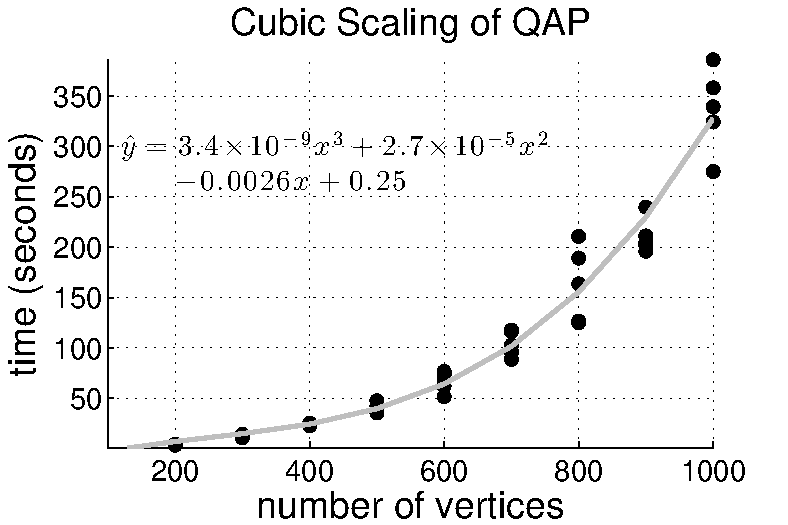
\includegraphics[width=0.7\linewidth]{ErdosRenyi_results.pdf}
	\caption{Running time of \FAQ~ as function of number of vertices. Data was sampled from an Erd\"os-R\'enyi model with $p=log(n)/n$.  Each dot represents a single simulation, with 100 simulations per $n$.  The solid line is the best fit cubic function.  Note the leading constant is $\dot{\approx} 10^{-9}$ seconds. \FAQ~ finds the optimal objective function value in every simulation.}
	\label{fig:scaling}
\end{figure}

% subsection algorithm_complexity_and_leading_constants (end)

\subsection{QAP Benchmark Accuracy} % (fold)
\label{sub:qap_benchmarks}

Having demonstrated both theoretically and empirically the \FAQ~ has cubic time complexity, we next decided to evaluate its accuracy on a suite of standard benchmarks.  More specifically, QAPLIB is a library of 137 quadratic assignment problems, ranging in size from 10 to 256 vertices \cite{Burkard1997}.  Recent graph matching papers typically evaluate the performance of their algorithm on 16 of the benchmarks that are known to be ``particularly difficult'' \cite{Zaslavskiy2009,Schellewald2001}.  We compare the results of \FAQ~ to the results of four other state-of-the-art graph matching algorithms: (1) the \Path~ algorithm, which solves a path between a convex and concave relaxation of QAP \cite{Zaslavskiy2009}, (2) \Qcv~ which is the convex relaxation used to initialize the \Path~ algorithm, (3) the \Rank~algorithm \cite{Singh2007}, which uses a spectral decomposition, and (4)  the Umeyama algorithm (denoted by \texttt{U} henceforth), which also uses a spectral decomposition \cite{Umeyama1988}.  We chose these four algorithms to compare because the code is freely available from the \texttt{graphm} package \cite{Zaslavskiy2009}.  
% Table \ref{tab:1} shows the results of these 5 algorithms on all 137 benchmarks, along with the optimal values (when they are available).  
Figure \ref{fig:allRelAccuracy} plots the logarithm (base 10, here and elsewhere) of the relative accuracy, that is, $\log_{10}(\mh{f}_{FAQ}/\mh{f}_X)$, for $X \in \{$\texttt{PATH, QCV, RANK, U, all}$\}$, where \texttt{all} is just the best performer of all the non \FAQ~ algorithms.  Clearly, \FAQ~ does significantly better than all the other algorithms, outperforming all of them on $\approx 94\%$ of the problems, often by nearly an order of magnitude in terms of relative error.
% Table \ref{tab:1} in the appendix shows the actual objective function values for all the algorithms on each problem.

\begin{figure}[htbp]
	\centering
		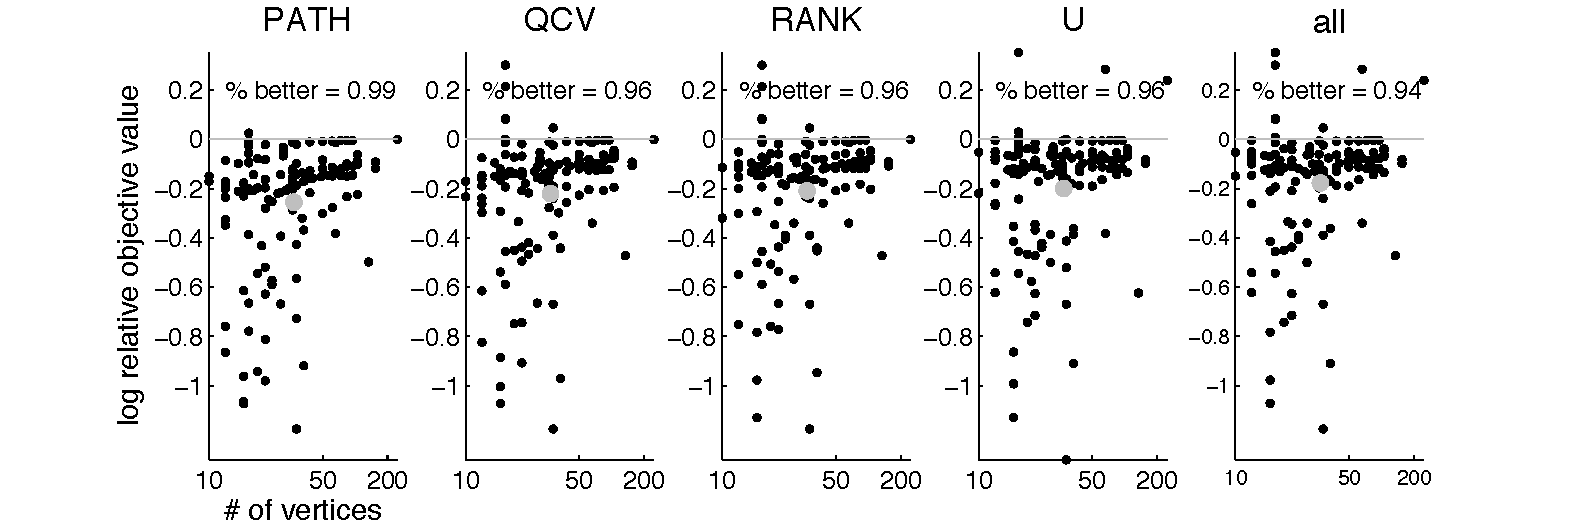
\includegraphics[width=1.0\linewidth]{allRelAccuracy.pdf}
	\caption{Relative accuracy---defined to be $\log_{10}(\mh{f}_{FAQ}/\mh{f}_X)$---of all the four algorithms compared with \FAQ.  Note that \FAQ~ is better than all the other algorithms on $\approx 94\%$ of the benchmarks. The abscissa is the log number of vertices.  The gray dot indicates the mean improvement of \FAQ~ over the other algorithms.}
	\label{fig:allRelAccuracy}
\end{figure}


% subsection qap_benchmarks (end)

\subsection{QAP Benchmark Efficiency} % (fold)
\label{sub:efficiency}


As we mentioned in the introduction, the quality of an \emph{approximate} algorithm depends not just on its accuracy, but also its efficiency.  Therefore, we compare the wall time of each of the five algorithms on all 137 benchmarks in Figure \ref{fig:allEfficiency}.  We fit an iteratively weighted least squares linear regression function (Matlab's \texttt{robustfit}) to regress the logarithm of time (in seconds) onto the logarithm of the number of vertices.  The numbers beside the lines indicate the slopes of the regression functions.  The \Path~ algorithm has the worst slope.  \Qcv~ and \FAQ~ have nearly identical slopes, which makes sense, given that the are solving very similar objective functions.  Similarly, \Rank~and \texttt{U} have very similar slopes; they are both using spectral approaches.  Note, however, that although the slope of \Rank~and \texttt{U} are smaller than that of \FAQ, they both seem to be super linear on this log-log plot, suggesting that as the number of vertices increases, their compute time might exceed that of the other algorithms.  Regardless, when comparing approximation algorithms, it is the speed/accuracy trade-off that is most important, in particular, in the problem space of interest.  For graphs with hundreds of vertices, all of these algorithms are sufficiently fast to use, so performance in terms of speed will be the deciding factor for many applications.  Of note is that the \FAQ~ algorithm has a relatively high variance for these problems.  This is due to the number of Hungarian algorithms performed, which is determined by the ``difficulty'' of the problem to converge.  We could fix the number of Hungarian algorithms, in which case the variance would decrease dramatically.  For our application, this variance is not problematic.

\begin{figure}[htbp]
	\centering
		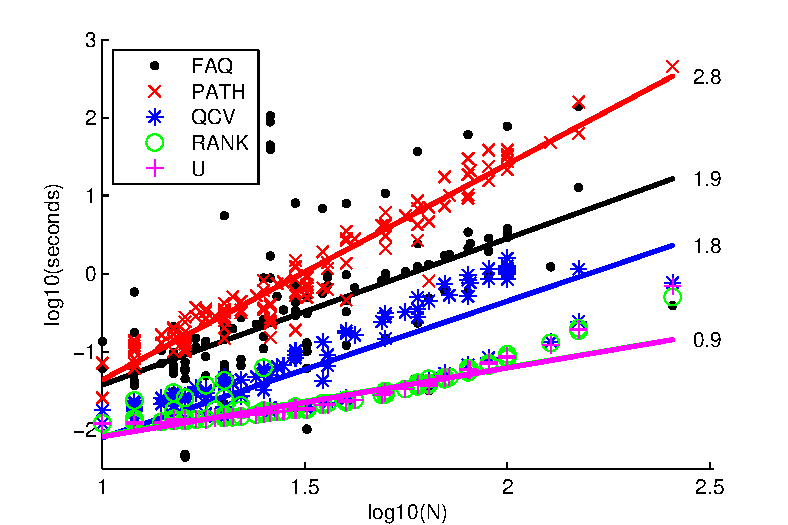
\includegraphics[height=3in]{allEfficiency.pdf}
	\caption{Absolute wall time for running each of the five algorithms on all 137 benchmarks. We fit a line on this log-log plot for each algorithm; the slope is displayed beside each line. The \FAQ~ slope is much better than the \Path~ slope, and worse than the others.  Note, however, the time for \Rank~and \texttt{U} appears to be superlinear on this log-log plot, suggesting that perhaps as the number of vertices increases, \Path~ might be faster. }
	\label{fig:allEfficiency}
\end{figure}


% subsection subsection_name (end)

\subsection{QAP Benchmark Accuracy/Efficiency Trade-off} % (fold)
\label{sub:tradeoff}


In the \Path, the authors demonstrated that \Path~ outperformed \Qcv~ and \texttt{U} on a variety of simulated and real examples in terms of objective function \cite{Zaslavskiy2009}.  If \FAQ~ yields a lower objective function value than \FAQ, and is faster, then it clearly is superior to \Path~ on such problems.  Figure \ref{fig:tradeoff} compares the performance of \FAQ~ with \Path~ along both dimensions of performance---accuracy and efficiency---for all 137 benchmarks in the QAPLIB library.  The right panel indicates that \FAQ~ is both more accurate and more efficient on $80\%$ of the problems.

\begin{figure}[htbp]
	\centering
		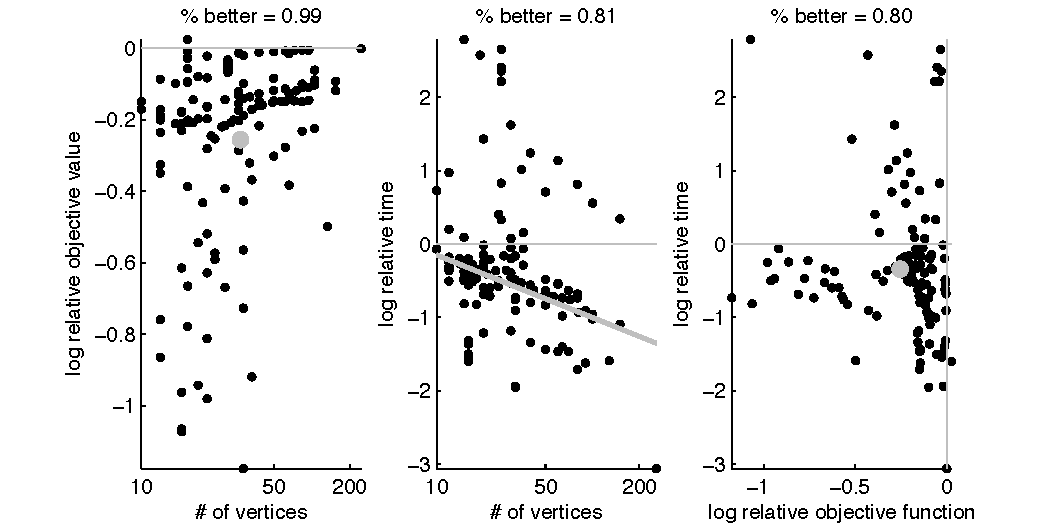
\includegraphics[width=1.0\linewidth]{allPathCompare.pdf}
	\caption{Comparison of \FAQ~ with \Path~ in terms of both accuracy and efficiency.  The left panel is the same as the left panel of Figure \ref{fig:allRelAccuracy}.  The middle plots the relative wall time of \FAQ~ to \Path~ as a function of the number of vertices, also on a log-log scale.  The gray line is the best fit slope on this plot, suggesting that \FAQ~ is getting exponentially faster than \Path~ as the number of vertices gets larger.  Finally, the right panel plots log relative time versus log relative objective function value, demonstrating that \FAQ~ outperforms \Path~ on both dimensions on $80\%$ of the benchmarks.}
	\label{fig:tradeoff}
\end{figure}





\subsection{QAP Directed Benchmarks}
\label{sub:directed}


Recently, Liu et al. \cite{Liu2012} proposed a modification of the \Path~ algorithm that adjusted \Path~ to be more appropriate for directed graphs, as the theory motivating the development of \Path~ relied upon the graphs being undirected.  \FAQ, on the other hand, does not depend on the graphs being simple; rather, directed or weighted graphs are both unproblematic. 
% a modification of the \Path~ algorithm arose that  Nothing in the development of our algorithm depends on the graphs being simple; indeed, \FAQ~ applies equally well to directed graphs.  To assess the performance of \FAQ~ on directed graphs, we compare the performance of our algorithm to the previous state-of-the-art. Liu et al.  recently developed an extended path following algorithm for directed graphs \cite{Liu2012}.
Liu et al. compare the performance of their algorithm (\Epath) with \texttt{U}, \Qcv, and \Grad~ on the set of 16 particularly difficult directed benchmarks from QAPLIB.  The \Epath~algorithm achieves at least as low objective value as the other algorithms on 15 of 16 benchmarks.  Our algorithm, \FAQ, always gets the best of the five algorithms.  Table \ref{tab:directed} shows the numerical results comparing \FAQ~ to \Epath~and \Grad, which sometimes did better than \Epath.  Note that some of the algorithms achieve the absolute minimum on some benchmarks.  
% Figure \ref{fig:lipa16} compares \FAQ~ to whichever other algorithm did best, clearly indicating that \FAQ~ is the best on these benchmarks.


\begin{table}[h!]
\caption{Comparison of \FAQ~ with optimal objective function value and previous state-of-the-art for directed graphs.  The best (lowest) value is in \textbf{bold}. Asterisks indicate achievement of the global minimum.  The number of vertices for each problem is the number in its name (second column).}
\begin{center}
\begin{tabular}{|r|r|r||l|l|l|l|l|}
	\hline 
	          \# &  Problem &      Optimal & \FAQ~ & \Epath~& \Grad~ \\
	\hline 
	           1 &  lipa20a &     3683 & \textbf{3791} &     3885 &     3909 \\ 
	           2 &  lipa20b &    27076 & \textbf{27076}$^*$ &    32081 &    \textbf{27076}$^*$ \\ 
	           3 &  lipa30a &    13178 & \textbf{13571} 	&    13577 &    13668 \\ 
	           4 &  lipa30b &   151426 & \textbf{151426}$^*$ & \textbf{151426}$^*$ &   \textbf{151426}$^*$ \\ 
	           5 &  lipa40a &    31538 & \textbf{32109} 	&    32247 &    32590 \\ 
	           6 &  lipa40b &   476581 & \textbf{476581}$^*$ &   \textbf{476581}$^*$ &   \textbf{476581}$^*$ \\ 
	           7 &  lipa50a &    62093 & \textbf{62962} &    63339 &    63730 \\ 
	           8 &  lipa50b &  1210244 & \textbf{1210244}$^*$ &  \textbf{1210244}$^*$ &  \textbf{1210244}$^*$ \\ 
	           9 &  lipa60a &   107218 & \textbf{108488} &   109168 &   109809 \\ 
	          10 &  lipa60b &  2520135 & \textbf{2520135}$^*$ &  \textbf{2520135}$^*$ &  \textbf{2520135}$^*$ \\ 
	          11 &  lipa70a &   169755 & \textbf{171820} &   172200 &   173172 \\ 
	          12 &  lipa70b &  4603200 & \textbf{4603200}$^*$ &  \textbf{4603200}$^*$ &  \textbf{4603200}$^*$ \\ 
	          13 &  lipa80a &   253195 & \textbf{256073} &   256601 &   258218 \\ 
	          14 &  lipa80b &  7763962 & \textbf{7763962}$^*$ &  \textbf{7763962}$^*$ &  \textbf{7763962}$^*$ \\ 
	          15 &  lipa90a &   360630 & \textbf{363937} &   365233 &   366743 \\ 
	          16 &  lipa90b & 12490441 & \textbf{12490441}$^*$ & \textbf{12490441}$^*$ & \textbf{12490441}$^*$ \\ 
	\hline
	\end{tabular}
\end{center}
\label{tab:directed}
\end{table}%


% \begin{figure}[htbp]
% 	\centering
% 		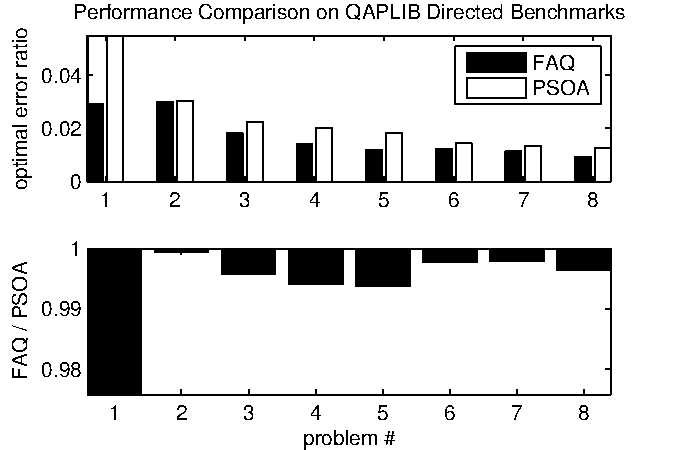
\includegraphics[width=0.5\linewidth]{lipa16.pdf}
% 	\caption{Performance of \FAQ~ relative to the previous state-of-the-art (\texttt{PSOA}) algorithms on the undirected QABLIB benchmarks. Top and Bottom panels as in Figure \ref{fig:path16}.  Note that \FAQ~ gets closer to the minimum on all 8 benchmarks for which the \FAQ~ and \texttt{PSOA} answer differ.}
% 	\label{fig:lipa16}
% \end{figure}
% 


\subsection{Theoretical properties of \FAQ} % (fold)
\label{sub:theory}

% Although we have no theorems proving error bounds on \FAQ~ relative to the optimal solution, we do have a number of theoretical results to buttress the numerical ones.  As mentioned above in \S \ref{sub:const}, \FAQ~ is a cubic-time algorithm, as its computational bottleneck is solving the LAPs, which are solved in $\mc{O}(n^3)$ by various algorithms collectively referred to as the ``Hungarian algorithm'' \cite{Jonker1987, Burkard2009}.   

In addition to guarantees on computational time, we have a guarantee on performance:  
\begin{lem}
	If $A$ and $B$ are the adjacency matrices of simple graphs (symmetric, hollow, and binary) that are isomorphic to one another, then the minimum of rQAP is equal to the minimum of QAP.
\end{lem}
\begin{proof}
Because any feasible solution to GM is also a feasible solution to rQAP, we must only show that the optimal objective function value to rQAP can be no better than the optimal objective function value of QAP.  Let $A=PBP\T$, so that $\langle A, PBP\T\rangle=2m$, where $m$ is the number of edges in $A$.  If rQAP could achieve a lower objective value, then it must be that there exists a $D \in \mc{D}$ such that $\langle A, DBD\T\rangle > \langle A, PBP\T\rangle = 2m$ (remember that we are minimizing the negative Euclidean inner product). For that to be the case, it must be that $(DBD\T)_{uv} \geq 1$ for some $(u,v)$.  That this is not so may be seen by the submultiplicativity of the norm induced by the $\ell_{\infty}$ norm:
$\norm{Dx}_\infty \leq \norm{D}_{\infty,\infty} \norm{x}_\infty$.  Applying this twice (once for each doubly stochastic matrix multiplication) yields our result.
% Consider $d_i=\langle D, \text{col}_i(BD\T) \rangle$, where $\text{col}_i(\cdot)$ indicates the $i^{th}$ column of the matrix.  $d_i \leq 1$ for all $i \in [n]$, therefore, our result holds.
\end{proof}
% subsection rQAP_solves_qap_ (end)


% section theoretical_results (end)

% \section{Numerical Results} % (fold)
% \label{sub:numerical_results}


% subsection numerical_results (end)


\subsection{Multiple Restarts} % (fold)
\label{sub:multiple_restarts}




Although \FAQ~ outperformed all other algorithms on nearly every benchmark, that \FAQ~ was not always the best was annoying to us.
% . \texttt{PSOA} on 13 of 16 undirected benchmarks, and always did the best amongst 16 of 16 directed benchmarks, it was annoying to us that we did not do best on all 32 benchmarks.  
% Note that the computational bottleneck of both \FAQ~ and \Path~ is the Hungarian algorithm which solves a LAP. 
% \FAQ~ strives to solve a non-convex problem.
% In \Path, the algorithm finds the minimum of a convex path between two extremes, $F_0$ and $F_1$.  Similarly, \texttt{QBP} finds the minimum of a convex program.  Our approach, on the other hand, does not construct a convex problem to solve, rather, it chooses an initial starting point and then finds a local optimum (note that the initial position of the \Path~ algorithm could also be variable, because $F_0$ is not convex as they assert, so their starting point depends on their initialization). 
% 
We therefore utilized the non-convexity of rQAP is as a feature, although it can equally well be regarded as a bug  (because rQAP is non-convex so the solution found by \FAQ~ depends on the initial condition).  We can utilize the non-convexity as a feature, however, whenever (i) we have some reason to believe that better solutions exist (many algorithms efficiently compute relatively tight lower bounds \cite{Anstreicher2009}), and (ii) we can efficiently search the space of initial conditions.  Although we lack any supporting theory of optimality, we do know how to sample feasible starting points.  Specifically, we desire that our starting points are ``near'' the doubly flat matrix, and satisfy the conditions.  Therefore, we  sample $K \in \mc{D}$, a random doubly stochastic matrix using 10 iterations of Sinkhorn balancing \cite{Sinkhorn1964}, and let our initial guess be $P^{(0)}=(J+K)/2$, where $J$ is the doubly flat matrix.  We can therefore use any number of restarts with this approach.  Fixing the number of restarts, we still have a cubic time algorithm, although the constants change.  

Table \ref{tab:restarts} shows the performance of running \FAQ~ 3 and 100 times, reporting only the best result (indicated by \FAQ$_3$ and \FAQ$_{100}$, respectively), and comparing it to the best performing result of the five algorithms (running only \FAQ~ once). Note that we only consider the 16 particularly difficult benchmarks for this evaluation. \FAQ~ only required three restarts to outperform all other approximate algorithms on all 16 of 16 difficult benchmarks.  Moreover, after 100 restarts, \FAQ~ finds the absolute minimum on 3 of the 16 benchmarks; none of the other algorithms ever achieved the absolute minimum on any of these benchmarks. 
% Figure \ref{fig:restarts} graphically demonstrates these results. 
 % Note that restarting \FAQ~ a fixed number of multiple times is still cubic.  Future work could investigate performance as a function of the number of restarts. %, although with an arbitrary number of random restarts, stating that it is cubic is somewhat meaningless.  



\begin{table}[h!]
\caption{Comparison of \FAQ~ with optimal objective function value and the best result  on the undirected benchmarks.  Note that \FAQ~ restarted 100 times finds the optimal objective function value in 3 of 16 benchmarks, and that \FAQ~ restarted 3 times finds a minimum better than the previous state-of-the-art on all 16 particularly difficult benchmarks.}
\begin{center}
\begin{tabular}{|r|r|r||l|l|l|l|l|}
\hline
\# & Problem  &   Optimal    & \FAQ$_{100}$ & \FAQ$_{3}$ & previous min \\
\hline
1&    chr12c &   11156 &    \textbf{12176} &   13072 & 13072 \\
2&    chr15a &    9896 &    \textbf{9896}$^*$ &   17272 &  19086 \\
3&    chr15c &    9504 &    \textbf{10960} &   14274 &  16206 \\
4&   chr20b &    2298 &     \textbf{2786} &    3068 &    3068 \\
5&    chr22b &    6194 &    \textbf{7218} &    7876 &   8482 \\
6&    esc16b & 	292 & 		\textbf{292}$^*$ & 294 &    296 \\
7& 	   rou12 &  235528 &  \textbf{235528}$^*$ &  238134 &    253684 \\
8& 	   rou15 &  354210 &  \textbf{356654} &  371458 &    371458 \\
9&      rou20 &  725522 &  \textbf{730614} &  743884 &    743884 \\
10&    tai10a &  135028 &  \textbf{135828} &  148970 &    152534 \\
11&    tai15a &  388214 &  \textbf{391522} &  397376 &    397376 \\
12&    tai17a &  491812 &  \textbf{496598} &  511574 &    529134 \\
13&    tai20a &  703482 &  \textbf{711840} &  721540 &    734276 \\
14&    tai30a & 1818146 & \textbf{1844636} & 1890738 &  1894640 \\
15&    tai35a & 2422002 & \textbf{2454292} & 2460940 &  2460940 \\
16&    tai40a & 3139370 & \textbf{3187738} & 3194826 &  3227612 \\
    \hline
\end{tabular}
\end{center}
\label{tab:restarts}
\end{table}%

% \begin{figure}[htbp]
% 	\centering
% 		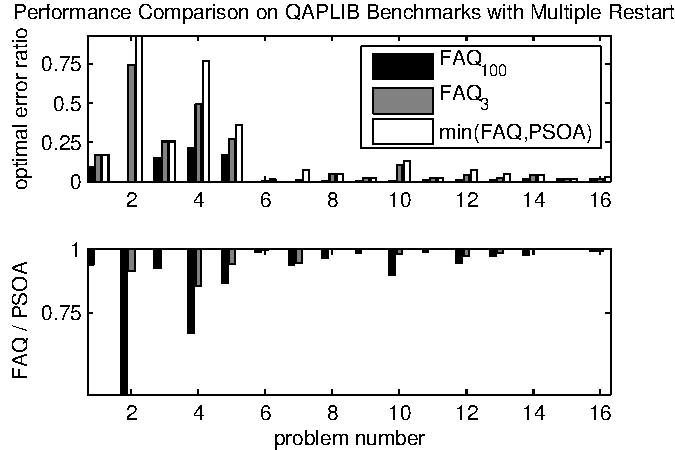
\includegraphics[width=0.5\linewidth]{path16_restarts.pdf}
% 	\caption{Performance of \FAQ~ with multiple restarts on the undirected benchmarks. \FAQ$_3$ yields a lower objective function value than the best result from Figure \ref{fig:path16}, and \FAQ$_{100}$ finds the absolute optimal permutation on 3 of the 16 benchmarks.  Note that no other algorithm compared ever found the optimal for any of the benchmarks.}
% 	\label{fig:restarts}
% \end{figure}


% subsection multiple_restarts (end)

% 
% \begin{figure}[htbp]
% 	\centering			
% 	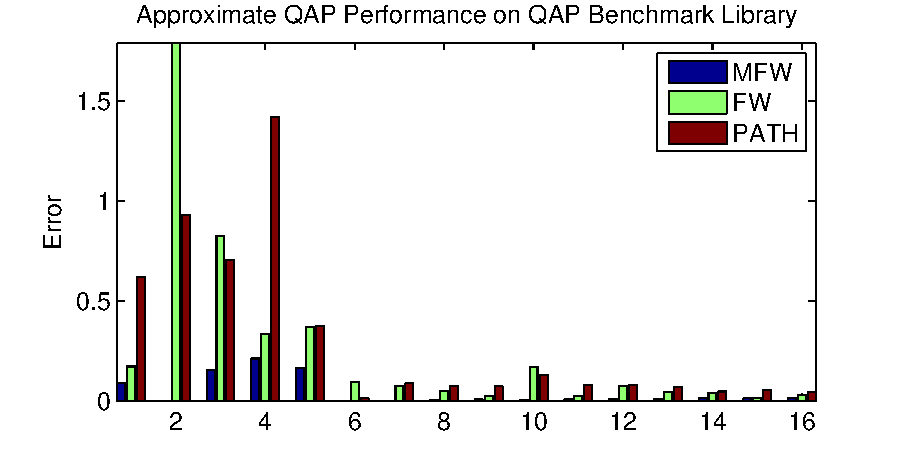
\includegraphics[width=1.0\linewidth]{benchmarks.pdf}
% 	\caption{\FAQ$_3$ outperforms the previous state-of-the-art (PSOA) on all 16 benchmark graph matching problems.  Moreover, \FAQa outperforms PSOA on 12 of 16 tests.  For 3 of 16 tests, \FAQb achieves the minimum (none of the other algorithms ever find the absolute minimum), as indicated by a black dot.  Let $f_*$ be the minimum and $\mh{f}_x$ be the minimum achieved by algorithm $x$.  Error is $\mh{f}_x/f_*-1$.  }
% 	\label{fig:fwpath}
% \end{figure}



\subsection{Brain-Graph Matching} % (fold)
\label{sub:connectome}




A ``chemical connectome'' is a brain-graph in which vertices correspond to (collections of) neurons, and edges correspond to chemical synapses between them. The \emph{Caenorhabditis elegans} (\emph{C. elegans}) is a small worm (nematode) with $302$ labeled vertices (in the hermaphroditic sex).  We consider the subgraph with $279$ somatic neurons that form edges with other neurons \cite{WhiteBrenner86, Varshney2011}.  
% Though vertices in brain-graphs can connect via either chemical or electrical synapses, the chemical connectome is the connectome of primary interest

% Two distinct kinds of edges exist between vertices: chemical and electrical ``synapses'' (edges). Any pair of vertices may have several edges of each type. Moreover, some of the synapses are hyper-edges amongst more than two vertices.  
Because pairs of neurons sometimes have multiple synapses between them, and they are directed, the chemical connectome of \emph{C. elegans} may be thought of as a weighted directed graph.
 % Thus, the connectome of a \emph{C. elegans} may be thought of as a weighted multi-hypergraph, where the weights are the number of edges of each type.  \FAQ~ natively operates on weighted or unweighted graphs.  
We therefore conducted the following synthetic experiments.  
Let $A_{uv} \in \{0,1,2,\ldots\}$ be the number of synapses from neuron $u$ to neuron $v$, and let $A=\{A_{uv}\}_{u,v \in [279]}$.  To generate synthetic data, we let $B^{(k)}=Q^{(k)} A {Q^{(k)}}\T$, for some $Q^{(k)}$ chosen uniformly at random from $\mc{P}$, effectively shuffling the vertex labels of the connectome.  Then, we try to graph match $A$ to $B^{(k)}$, for  $k =1,2,\ldots, 1000$, that is, we repeat the experiment $1000$ times.  We define accuracy as the fraction of vertices correctly assigned. We always start with the doubly flat matrix.


\begin{figure}[htbp]
	\centering
		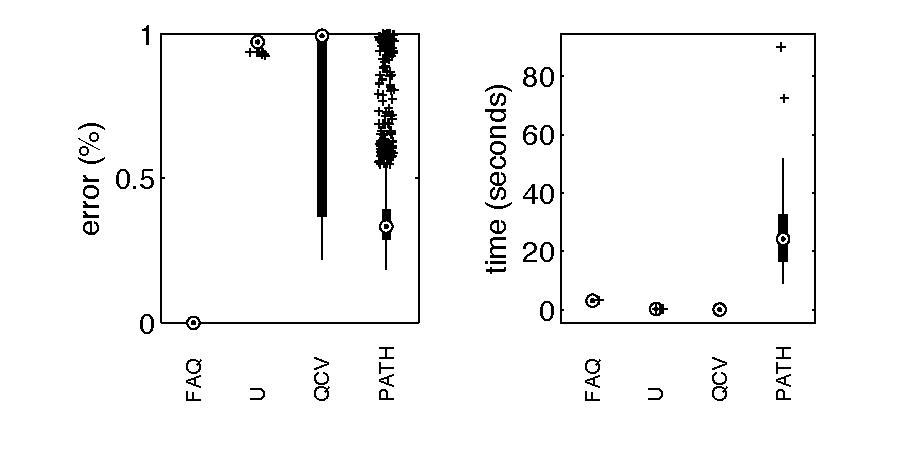
\includegraphics[width=0.7\linewidth]{chemicalConnectome.pdf}
	\caption{Performance of \texttt{U}, \Qcv, \Path, and \FAQ~ on synthetic C.~elegans connectome data, that is, graph matching the true connectomes with permuted versions of themselves.  Error is the fraction of vertices correctly matched.  Circle indicates the median, thick black bars indicate the quartiles, thin black lines indicate extreme but non-outlier points, and plus signs are outliers. The left panel indicate error (fraction of misassigned vertices), and the right panel indicates wall time on a 2.2 GHz Apple MacBook.   \FAQ~ always obtained the optimal solution, whereas none of the other algorithms ever found the optimal.    \FAQ~ also ran very quickly, nearly as quickly as \texttt{U} and \Qcv, and much faster than \Path, even though the \FAQ~ implementation is in Matlab, and the others are in C.}
	\label{fig:connectomes}
\end{figure}


Figure \ref{fig:connectomes} displays the results of \FAQ~ along with \texttt{U}, \Qcv,  and \Path.  The left panel indicates that \FAQ~ \emph{always} found the optimal solution for the chemical connectome, whereas none of the other algorithms \emph{ever} found the optimal solution.  The right panel compares the wall time of the various algorithms, running on an 2.2 GHz Apple MacBook. Note that we have only a Matlab implementation of \FAQ, whereas the other algorithms are implemented in C.  Unlike in the QAPLIB benchmarks, \FAQ~ runs nearly as quickly as both \texttt{U} and \Qcv; and as expected, \FAQ~ runs significantly faster than \Path.  
%This suggests that lower level language implementation of \FAQ~ might be 

% The properties of this connectomes are analyzed in \cite{Varshney2011}; a cursory evaluation of the properties of these graphs does not suggest to us why the chemical connectome was so much easier to graph match than the electrical one. 


To investigate the performance of \FAQ~ on undirected graphs, we ran \FAQ~ on binarized symmeterized versions of the graphs ($A_{uv}=1$ if and only if $A_{uv}\geq 1$ or $A_{vu} \geq 1$).  The resulting errors are nearly identical to those presented in Figure \ref{fig:connectomes}, although speed increased by greater than a factor of two. Note that the number of vertices in this brain-graph matching problem---279---is larger than the largest of the 137 benchmarks used above. 




\section{Discussion}
\label{sec:discussion}

\subsection{Summary}

This work presents a fast approximate quadratic assignment problem algorithm called \FAQ~ for approximately solving large quadratic assignment problems, motivated by brain-graph matching.  Our key insight was to relax the binary constraint of QAP to its continuous and non-negative counterpart---the doubly stochastic matrix---which is the convex hull of the original feasible region.  
We demonstrated that not only is \FAQ~ cubic in time, but also its leading constants are quite small---$10^{-9}$---suggesting that it can be used for graphs with hundreds or thousands of vertices (\S \ref{sub:const}).  

Moreover, it achieves better accuracy than previous state-of-the-art approximate algorithms on on over $93\%$ of the 137 QAPLIB benchmarks (\S \ref{sub:qap_benchmarks}), is faster than \Path (\S \ref{sub:efficiency}), and is both faster and achieves at least as low performance on over $80\%$ of the benchmarks (\S \ref{sub:tradeoff}),  including both directed and undirected graph matching problems (\S \ref{sub:directed}).  
In addition to the theoretical guarantees of cubic run time, we also demonstrate that the solution to our relaxed optimization problem, rQAP, is identical to that for QAP whenever the two graphs are simple and isomorphic to one another (\S \ref{sub:theory}).
Because rQAP is non-convex, we also consider multiple restarts, and achieve improved performance for the particularly difficult benchmarks using only two or three restarts (\S \ref{sub:multiple_restarts}).  

  
Finally, we used it to match C.~elegans connectomes to permuted versions of themselves (\S \ref{sub:connectome}). Of the four state-of-the-art algorithms considered, \FAQ~ achieved perfect performance $100\%$ of the time, whereas none of the other three algorithms ever achieved perfect performance.  Moreover, \FAQ~ ran about as fast as two of them, and significantly faster than \Path, even though \FAQ~ is implemented in Matlab, and the others are implemented in C.  Note that these connectomes have 279 vertices, more vertices than even the largest benchmarks. 



\subsection{Related Work}


Our approach is quite similar to other approaches that have recently appeared in the literature.  Perhaps its closest cousins include \cite{Zaslavskiy2009, Zaslavskiy2010} and \cite{Escolano2011}, which are all of the ``PATH'' following variety.  Zaslavskiy et al.    seems to consider but discard \FAQ~  \cite{Zaslavskiy2009} because they did not like projecting onto the set of permutations matrices.  Their solution, while elegant, is both slower and obtains a worse objective function value on nearly all benchmark problems.  Others have considered similar relaxations, but usually in the context of finding lower bounds  \cite{Anstreicher2001} or as subroutines for finding exact solutions \cite{Brixius2000}.  Our work seems to be the first to utilize the precise algorithm described in Pseudocode \ref{alg:1} to find fast approximate solutions to QAP.


\subsection{Future Work}

Fortunately, our work is not done. Even with very small leading constants for this algorithm, as $n$ increases, the computational burden gets quite high.  For example, extrapolating the curve of Figure \ref{fig:scaling}, this algorithm would take about 20 years to finish (on a standard laptop from 2011) when $n=100,000$.  We hope to be able to approximately solve rQAP on graphs much larger than that, given that the number of neurons even in a fly brain, for example, is $\approx 250,000$.  More efficient algorithms and/or implementations are required for such massive graph matching. Although a few other state-of-the-art algorithms were more efficient than \FAQ, their accuracy was significantly worse.  So the search continues to find approximate graph matching algorithms with scaling rules like \Qcv, \texttt{U} or \Rank, but performance like \FAQ.


Additional future work might generalize \FAQ~ in a number of ways.  First, many (brain-) graphs of interest will be errorfully observed \cite{Priebe2011}, that is, vertices might be missing and putative edges might exhibit both false positives and negatives.  Explicitly dealing with this error source is both theoretically and practically of interest \cite{VP11_unlabeled}.  
Second, for many brain-graph matching problems, the number of vertices will not be the same across the brains.  Recent work from \cite{Zaslavskiy2009, Zaslavskiy2010} and \cite{Escolano2011} suggest that extensions in this direction would be both relatively straightforward and effective. Third, the most ``costly'' subroutine is LAP.  Fortunately, LAP is a linear optimization problem with linear constraints.  A number of parallelized optimization strategies could therefore potentially be brought to bear on this problem \cite{Boyd2011}.  Fourth, our matrices have certain special properties, namely sparsity, which makes more efficient algorithms (such as ``active set'' algorithms) readily available for further speed increases.  Fifth, for brain-graphs, we have some prior information that could easily be incorporated in the form of vertex attributes.  For example, position in the brain, cell type, etc., could be used to measure ``dissimilarity'' between vertices.  %The WGMP could easily incorporate these dissimilarities, in fact, the original QAP formulation already encodes them via the matrix $C$; that matrix was simply dropped when WGMP was originally proposed.  
% The objective function could then be modified to give
% \begin{align} \label{eq:Jqap}
% 	\mt{Q}_{AB}= \argmin_{Q \in \mc{D}} \norm{Q A Q\T - B}^2_F + \lambda J(Q),
% \end{align}
% where $J(Q)$ is a dissimilarity based penalty and $\lambda$ is a hyper-parameter.  
Finally, although this approach natively operates on both unweighted and weighted graphs, multi-graphs are a possible extension.

\subsection{Concluding Thoughts}

In conclusion, this manuscript has presented an algorithm for approximately solving the quadratic assignment problem that is fast, effective, and easily generalizable.  Yet, the $\mc{O}(n^3)$ complexity remains too slow to solve many problems of interest.  To facilitate further development and applications, all the code and data used in this manuscript is available from the first author's website, \url{http://jovo.me}.




\appendix
\newpage

\clearpage
\section{Linear Assignment Problems} % (fold)
% \label{ssub:linear_assignment_problems}

% subsubsection linear_assignment_problems (end)

The standard way of writing a Linear Assignment Problem (LAP) is
\begin{equation*}
% \text{(LAP)} \qquad  
\begin{array}{cl}
			\text{minimize}   & \sum_{u,v \in [n]} a_{u \pi(v)} b_{uv} \\
			\text{subject to}  &P \in \mc{P}.   
\end{array} %\label{eq:LAP}
\end{equation*}
The LAP objective function, like the QAP objective function, enjoys a number of equivalent formulations, including
% , similar to the QAP objective function (cf Eq. \eqref{eq:equiv})
% \begin{multline} \label{eq:equiv}
% (a_{uv}-b_{\pi(u)\pi(v)})^2 = \norm{A - PBP\T}_F^2 \\ = tr \{ (A - PBP\T)\T (A - PBP\T)\}.
% \end{multline}
% 
% 
% which can be written equivalently in a number of ways using the notion of permutation matrix introduced in the main text, including
\begin{equation}
\text{(LAP)} \qquad  
\begin{array}{cl}
			\text{minimize}   & \langle P, AB\T \rangle \\
			\text{subject to}  &P \in \mc{P}.   
\end{array}\label{eq:LAP}
\end{equation}
% 
% \begin{subequations} \label{eq:LAP2}
% \begin{align}
% 	&\argmin_{\PmcP} \norm{PA - B}_F =\\
% 	&\argmin_{\PmcP} \, tr(PA-B)\T (PA-B)=\\ 
% 	% &\argmin_{\PmcP} tr (A\T P\T PA) - tr(2PAB\T) + tr(B\T B)=\\ 
% 	&\argmin_{\PmcP}  -tr (P AB\T) = \argmin_{\PmcP}  -\langle P\T, AB\T \rangle = \label{eq:2c} \\
% 	% &\argmin_{\PmcP}  -\sum_{u,v \in [n]} p_{ij} a_{ij} b_{ji}
% 	% =\\% &\argmin_{\PmcP}  - \text{vec}(P)\T \text{vec}(AB\T).=\\
% 	&\argmin_{\PmcP}  -\langle P, AB\T \rangle, \label{eq:dotLAP}
% \end{align}
% \end{subequations}
% where $\langle \cdot,\cdot \rangle$ %the equality on the second to last line defines is the usual Euclidean inner product, i.e., $\langle X,Y\rangle \defn tr(X\T Y)= \sum_{ij} x_{ij} y_{ij}$.
% While the objective function and the first two constraints of LAP are linear, t
The binary constraints of LAP---like those of QAP---make solving even this problem computationally tricky.  Nonetheless, in the last several decades, there has been much progress in accelerating algorithms for solving LAPs, starting with exponential time, all the way down to $\mc{O}(n^3)$ for general LAPs, and even faster for certain special cases (e.g., sparse matrices) \cite{Jonker1987, Burkard2009}.

% That Eq.~\eqref{eq:dir} is a LAP is evident by considering Eq.~\eqref{eq:dotLAP}.  
To see that Eq.~\eqref{eq:dir} is identical to Eq.~\eqref{eq:LAP}, 
simply let $A=\nabla_P^{(i)}$ and $B=I$ (the $n\times n$ identity matrix).


% The last form indicates that LAP is a linear programming problem (hence the name).  Yet, the constraints, $\mc{P}$, make it a bit trickier.  The feasible region $\mc{P}$ can be written as a set of three constraints: two linear equality constraint sets and a binary constraint.  The LAP objection function with constraints can explicitly be written:
% \begin{align}
% 		&\text{minimize}_P  &&\sum_{u \in \mc{V}} -p_{ij} a_{ij} b_{ji} \nonumber \\
% 		&\text{subject to } && \sum_{u \in \mc{V}} p_{ij} = 1 \, \forall u \in \mc{V} \nonumber \\
% 		& && \sum_{v \in \mc{V}} p_{ij} = 1 \, \forall v \in \mc{V}, \nonumber \\
% 		& &&p_{ij} \in \{0,1\} \, \forall u,v. \label{eq:rLAP}	
% \end{align}
% Perhaps because LAP comes up in a wide variety of contexts, a large number of algorithms have been developed to solve LAP \cite{Burkard2009}.  These algorithms have become increasing efficient.  
% One of the most popular algorithms, the so-called ``Hungarian algorithm'' has time complexity $\mc{O}(n^3)$ \cite{Jonker1987}.  Under certain conditions (for example, when $AB\T$ is sparse), faster implementations are also available.  As will be seen below, LAP is a key subroutine to our inexact QAP solution.  

To solve a LAP, consider a continuous relaxation of LAP, specifically, relaxing the permutation matrix constraint to a doubly stochastic matrix constraint:
% A matrix $P$ is doubly stochastic precisely when $P$ satisfies the following three conditions: 
% \begin{enumerate}
% \item	$P\mb{1} = \mb{1}$,
% \item	$P\T \mb{1}=\mb{1}$, %\\
% \item 	$P \in  \Real_+^{n \times n}$,
% \end{enumerate}
% where the third constraint relaxes the binary constraints of the permutation matrices with a non-negativity constraint.  
% Let $\mc{D}$ be the set of doubly stochastic matrices.
% With this, we now state a relaxed LAP problem:
\begin{equation}
\text{(rLAP)} \qquad  
\begin{array}{cl}
			\text{minimize}   & \langle P, AB\T \rangle \\
			\text{subject to}  &P \in \mc{D}.   
\end{array}\label{eq:LAP}
\end{equation}
% \begin{subequations} \label{eq:rLAP}
% \begin{align}
% 		\text{(rLAP) } \quad &\underset{P}{\text{minimize}}  &&-\langle P, AB\T \rangle \\
% 		&\text{subject to } && P \in \mc{D}.
% 		% && \sum_{u \in \mc{V}} p_{ij} = 1 \, \forall u \in \mc{V} \nonumber \\
% 		% 		& && \sum_{v \in \mc{V}} p_{ij} = 1 \, \forall v \in \mc{V}, \nonumber \\
% 		% 		& &&p_{ij} \geq 0 \, \forall u,v, \label{eq:ALAP}	
% \end{align}
% \end{subequations}
As it turns out, the minima of LAP and rLAP are equal to one anther \cite{Burkard2009}.
% solving rLAP is equivalent to solving LAP.
% \begin{prop}
% 	LAP and rLAP are equivalent, meaning that they have the same optimal objective function value.
% \end{prop}
% \begin{proof}
% 	Although this proposition is typically proven by invoking total unimodularity, we present a  proof here that we find simpler.	Let $P^L$ be a solution to LAP and let $P^r = \sum_{i\in[k]} \alpha_i P_i$ be a solution to rLAP for some positive integer $k$, permutation matrices $\{P_i\}_{i \in [k]}$, and positive real numbers $\{\alpha_i\}_{i \in[k]}$ such that $\sum_{i \in [k]} \alpha_i=1$.  Note that it must be the case that
% \begin{align}
% 	\langle P^L, AB\T \rangle \geq \langle P^r, AB\T \rangle,
% \end{align}
% because $P^L$ is also a solution for rLAP. Expanding $P^r$, we have
% \begin{align}
% 	\langle P^r, AB\T \rangle = \langle \sum_i \alpha_i P_i, AB\T \rangle = \sum_i \alpha_i \langle  P_i, AB\T \rangle.
% \end{align}
% But we know that 
% \begin{align}
% 	\langle P^L, AB\T \rangle \leq \langle P, AB\T \rangle
% \end{align}
% for any $P \in \mc{P}$ because $P^L$ solves LAP, so  
% 	% 
% 	% 
% 	% \begin{multline}
% 	% \langle P^L,AB\T \rangle = \langle  \sum_{i\in[k]} \alpha_i P_i^L, AB\T \rangle=  \sum_{i\in[k]} \alpha_i \langle  P_i^L, AB\T \rangle	 \\
% 	% \leq \sum_{i\in[k]} \alpha_i \langle P^r, AB\T  \rangle = \langle P^r, AB\T \rangle \leq \langle P^L, AB\T \rangle,
% 	% \end{multline}
% 	% % then we have a contradiction, 
% 	% because $P^r$ is feasible in rLAP.
% 	\end{proof}
This relaxation motivates our approach to approximating QAP.

	



\section*{Acknowledgment}
% 
The authors would like to acknowledge 
% two helpful reviewers as well as 
Lav Varshney for providing the data. This work was partially supported by the Research Program in Applied Neuroscience. 
% 
% 

\bibliographystyle{model1-num-names}

 \begin{thebibliography}{42}
\expandafter\ifx\csname natexlab\endcsname\relax\def\natexlab#1{#1}\fi
\providecommand{\bibinfo}[2]{#2}
\ifx\xfnm\relax \def\xfnm[#1]{\unskip,\space#1}\fi
%Type = Article
\bibitem[{Koopmans et~al.(1957)Koopmans, Beckman, and Beckmann}]{Koopmans1957}
\bibinfo{author}{T.~C. T.~C. Koopmans}, \bibinfo{author}{M.~Beckman},
  \bibinfo{author}{M.~Beckmann},
\newblock \bibinfo{title}{{Assignment Problems and the Location of Economic
  Activities}},
\newblock \bibinfo{journal}{The Econometric Society} \bibinfo{volume}{25}
  (\bibinfo{year}{1957}) \bibinfo{pages}{53--76}.
%Type = Article
\bibitem[{Umeyama(1988)}]{Umeyama1988}
\bibinfo{author}{S.~Umeyama},
\newblock \bibinfo{title}{{An Eigendecomposition Approach to Weighted Graph
  Matching Problems}},
\newblock \bibinfo{journal}{Analysis} \bibinfo{volume}{I}
  (\bibinfo{year}{1988}).
%Type = Book
\bibitem[{Papadimitriou and Steiglitz(1998)}]{Papadimitriou1998}
\bibinfo{author}{C.~H. Papadimitriou}, \bibinfo{author}{K.~Steiglitz},
  \bibinfo{title}{{Combinatorial Optimization: Algorithms and Complexity}},
  \bibinfo{publisher}{Dover Publications}, \bibinfo{year}{1998}.
%Type = Article
\bibitem[{Conte et~al.(2004)Conte, Foggia, Sansone, and Vento}]{Conte2004}
\bibinfo{author}{D.~Conte}, \bibinfo{author}{P.~Foggia},
  \bibinfo{author}{C.~Sansone}, \bibinfo{author}{M.~Vento},
\newblock \bibinfo{title}{{Thirty Years of Graph Matching in Pattern
  Recognition}},
\newblock \bibinfo{journal}{International Journal of Pattern Recognition and
  Artificial Intelligence} \bibinfo{volume}{18} (\bibinfo{year}{2004})
  \bibinfo{pages}{265--298}.
%Type = Book
\bibitem[{Burkard et~al.(2009)Burkard, Dell'Amico, and Martello}]{Burkard2009}
\bibinfo{author}{R.~E. Burkard}, \bibinfo{author}{M.~Dell'Amico},
  \bibinfo{author}{S.~Martello}, \bibinfo{title}{{Assignment Problems}},
  \bibinfo{publisher}{SIAM}, \bibinfo{year}{2009}.
%Type = Book
\bibitem[{Kolaczyk(2010)}]{Kolaczyk2010}
\bibinfo{author}{E.~Kolaczyk}, \bibinfo{title}{{Statistical Analysis of Network
  Data: Methods and Models}}, \bibinfo{publisher}{Springer},
  \bibinfo{year}{2010}.
%Type = Article
\bibitem[{Sporns et~al.(2005)Sporns, Tononi, and Kotter}]{SpornsKotter05}
\bibinfo{author}{O.~Sporns}, \bibinfo{author}{G.~Tononi},
  \bibinfo{author}{R.~Kotter},
\newblock \bibinfo{title}{{The Human Connectome: A Structural Description of
  the Human Brain}},
\newblock \bibinfo{journal}{PLoS Computational Biology} \bibinfo{volume}{1}
  (\bibinfo{year}{2005}) \bibinfo{pages}{e42}.
%Type = Phdthesis
\bibitem[{Hagmann(2005)}]{Hagmann05}
\bibinfo{author}{P.~Hagmann}, \bibinfo{title}{{From diffusion MRI to brain
  connectomics}}, Ph.D. thesis, Institut de traitement des signaux,
  \bibinfo{year}{2005}.
%Type = Article
\bibitem[{Herculano-Houzel(2012)}]{Herculano-Houzel2012}
\bibinfo{author}{S.~Herculano-Houzel},
\newblock \bibinfo{title}{{The remarkable, yet not extraordinary, human brain
  as a scaled-up primate brain and its associated cost.}},
\newblock \bibinfo{journal}{Proceedings of the National Academy of Sciences of
  the United States of America} \bibinfo{volume}{109 Suppl}
  (\bibinfo{year}{2012}) \bibinfo{pages}{10661--8}.
%Type = Article
\bibitem[{Csernansky et~al.(2004)Csernansky, Wang, Joshi, Ratnanather, and
  Miller}]{Csernansky2004}
\bibinfo{author}{J.~G. Csernansky}, \bibinfo{author}{L.~Wang},
  \bibinfo{author}{S.~C. Joshi}, \bibinfo{author}{J.~T. Ratnanather},
  \bibinfo{author}{M.~I. Miller},
\newblock \bibinfo{title}{{Computational anatomy and neuropsychiatric disease:
  probabilistic assessment of variation and statistical inference of group
  difference, hemispheric asymmetry, and time-dependent change.}},
\newblock \bibinfo{journal}{NeuroImage} \bibinfo{volume}{23 Suppl 1}
  (\bibinfo{year}{2004}) \bibinfo{pages}{S56--68}.
%Type = Article
\bibitem[{Kubicki et~al.(2007)Kubicki, McCarley, Westin, Park, Maier, Kikinis,
  Jolesz, and Shenton}]{Kubicki2007}
\bibinfo{author}{M.~Kubicki}, \bibinfo{author}{R.~McCarley},
  \bibinfo{author}{C.-F. Westin}, \bibinfo{author}{H.-J. Park},
  \bibinfo{author}{S.~Maier}, \bibinfo{author}{R.~Kikinis},
  \bibinfo{author}{F.~A. Jolesz}, \bibinfo{author}{M.~E. Shenton},
\newblock \bibinfo{title}{{A review of diffusion tensor imaging studies in
  schizophrenia.}},
\newblock \bibinfo{journal}{Journal of Psychiatric Research}
  \bibinfo{volume}{41} (\bibinfo{year}{2007}) \bibinfo{pages}{15--30}.
%Type = Article
\bibitem[{Calhoun et~al.(2011)Calhoun, Sui, Kiehl, Turner, Allen, and
  Pearlson}]{Calhoun2011}
\bibinfo{author}{V.~D. Calhoun}, \bibinfo{author}{J.~Sui},
  \bibinfo{author}{K.~a. Kiehl}, \bibinfo{author}{J.~A. Turner},
  \bibinfo{author}{E.~a. Allen}, \bibinfo{author}{G.~Pearlson},
\newblock \bibinfo{title}{{Exploring the psychosis functional connectome:
  aberrant intrinsic networks in schizophrenia and bipolar disorder.}},
\newblock \bibinfo{journal}{Frontiers in psychiatry / Frontiers Research
  Foundation} \bibinfo{volume}{2} (\bibinfo{year}{2011}) \bibinfo{pages}{75}.
%Type = Article
\bibitem[{Fornito and Bullmore(2012)}]{Fornito2012}
\bibinfo{author}{A.~Fornito}, \bibinfo{author}{E.~T. Bullmore},
\newblock \bibinfo{title}{{Connectomic intermediate phenotypes for psychiatric
  disorders.}},
\newblock \bibinfo{journal}{Frontiers in psychiatry / Frontiers Research
  Foundation} \bibinfo{volume}{3} (\bibinfo{year}{2012}) \bibinfo{pages}{32}.
%Type = Article
\bibitem[{Fornito et~al.(2012)Fornito, Zalesky, Pantelis, and
  Bullmore}]{Fornito2012a}
\bibinfo{author}{A.~Fornito}, \bibinfo{author}{A.~Zalesky},
  \bibinfo{author}{C.~Pantelis}, \bibinfo{author}{E.~T. Bullmore},
\newblock \bibinfo{title}{{Schizophrenia, neuroimaging and connectomics}},
\newblock \bibinfo{journal}{NeuroImage}  (\bibinfo{year}{2012}).
%Type = Article
\bibitem[{Vogelstein and Priebe(2011)}]{VP11_unlabeled}
\bibinfo{author}{J.~T. Vogelstein}, \bibinfo{author}{C.~E. Priebe},
\newblock \bibinfo{title}{{Shuffled Graph Classification: Theory and Connectome
  Applications}},
\newblock \bibinfo{journal}{Submitted to IEEE PAMI}  (\bibinfo{year}{2011}).
%Type = Article
\bibitem[{Duin et~al.(2011)Duin, Pękalska, and Pękalskab}]{Duin2011}
\bibinfo{author}{R.~P.~W. Duin}, \bibinfo{author}{E.~Pękalska},
  \bibinfo{author}{E.~Pękalskab},
\newblock \bibinfo{title}{{The dissimilarity space: Bridging structural and
  statistical pattern recognition}},
\newblock \bibinfo{journal}{Pattern Recognition Letters} \bibinfo{volume}{in
  press} (\bibinfo{year}{2011}).
%Type = Article
\bibitem[{Fortin(1996)}]{Fortin1996}
\bibinfo{author}{S.~Fortin},
\newblock \bibinfo{title}{{The Graph Isomorphism Problem}},
\newblock \bibinfo{journal}{Technical Report, University of Alberta, Dept of
  CS}  (\bibinfo{year}{1996}).
%Type = Article
\bibitem[{Babali et~al.(1980)Babali, Erdős, and Selkow}]{Babai1980}
\bibinfo{author}{L.~Babali}, \bibinfo{author}{P.~Erdős},
  \bibinfo{author}{S.~M. Selkow},
\newblock \bibinfo{title}{{RANDOM GRAPH ISOMORPHISM}},
\newblock \bibinfo{journal}{SIAM Journal on Computing} \bibinfo{volume}{9}
  (\bibinfo{year}{1980}) \bibinfo{pages}{628--635}.
%Type = Article
\bibitem[{Babali(1981)}]{Babai1981}
\bibinfo{author}{L.~Babali},
\newblock \bibinfo{title}{{Moderately Exponential Bound for Graph
  Isomorphism}},
\newblock \bibinfo{journal}{Fundamentals of Computation Theory}
  (\bibinfo{year}{1981}) \bibinfo{pages}{34--50}.
%Type = Article
\bibitem[{Chen(1994)}]{Chen1994}
\bibinfo{author}{J.~Chen},
\newblock \bibinfo{title}{{A Linear-Time Algorithm for Isomorphism of Graphs of
  Bounded Average Genus}},
\newblock \bibinfo{journal}{SIAM Journal on Discrete Mathematics}
  \bibinfo{volume}{7} (\bibinfo{year}{1994}) \bibinfo{pages}{614}.
%Type = Article
\bibitem[{Frank and Wolfe(1956)}]{Frank1956}
\bibinfo{author}{M.~Frank}, \bibinfo{author}{P.~Wolfe},
\newblock \bibinfo{title}{{An Algorithm for Quadratic Programming}},
\newblock \bibinfo{journal}{Naval Research Logistics Quarterly}
  \bibinfo{volume}{3} (\bibinfo{year}{1956}) \bibinfo{pages}{95--110}.
%Type = Book
\bibitem[{Bradley et~al.(1977)Bradley, Hax, and Magnanti}]{Bradley1977}
\bibinfo{author}{S.~P. Bradley}, \bibinfo{author}{A.~C. Hax},
  \bibinfo{author}{T.~L. Magnanti}, \bibinfo{title}{{Applied Mathematical
  Programming}}, \bibinfo{publisher}{Addison-Wesley}, \bibinfo{year}{1977}.
%Type = Article
\bibitem[{Anstreicher(2003)}]{Anstreicher03}
\bibinfo{author}{K.~M. Anstreicher},
\newblock \bibinfo{title}{{Recent advances in the solution of quadratic
  assignment}},
\newblock \bibinfo{journal}{SIAM Journal on Optimization} \bibinfo{volume}{97}
  (\bibinfo{year}{2003}) \bibinfo{pages}{27--42}.
%Type = Article
\bibitem[{Kuhn(1955)}]{Kuhn1955}
\bibinfo{author}{H.~W. Kuhn},
\newblock \bibinfo{title}{{The Hungarian method for the assignment problem}},
\newblock \bibinfo{journal}{Naval Research Logistics Quarterly}
  \bibinfo{volume}{2} (\bibinfo{year}{1955}) \bibinfo{pages}{83--97}.
%Type = Article
\bibitem[{Kőnig(1931)}]{Konig1931}
\bibinfo{author}{D.~Kőnig},
\newblock \bibinfo{title}{{Gr\'{a}fok \'{e}s M\'{a}trixok}},
\newblock \bibinfo{journal}{Matematikai \'{e}s Fizikai Lapok}
  \bibinfo{volume}{38} (\bibinfo{year}{1931}) \bibinfo{pages}{116--119}.
%Type = Article
\bibitem[{Egev\'{a}ry(1931)}]{Egevary1931}
\bibinfo{author}{J.~Egev\'{a}ry},
\newblock \bibinfo{title}{{Matrixok kombinatorius tulajdons\'{a}gair\'{o}l}},
\newblock \bibinfo{journal}{Matematikai \'{e}s Fizikai Lapok}
  \bibinfo{volume}{38} (\bibinfo{year}{1931}) \bibinfo{pages}{16--28}.
%Type = Article
\bibitem[{Jonker and Volgenant(1987)}]{Jonker1987}
\bibinfo{author}{R.~Jonker}, \bibinfo{author}{A.~Volgenant},
\newblock \bibinfo{title}{{A shortest augmenting path algorithm for dense and
  sparse linear assignment problems}},
\newblock \bibinfo{journal}{Computing} \bibinfo{volume}{38}
  (\bibinfo{year}{1987}) \bibinfo{pages}{325--340}.
%Type = Article
\bibitem[{Burkard et~al.(1997)Burkard, Karisch, and Rendl}]{Burkard1997}
\bibinfo{author}{R.~E. Burkard}, \bibinfo{author}{S.~E. Karisch},
  \bibinfo{author}{F.~Rendl},
\newblock \bibinfo{title}{{QAPLIB – A Quadratic Assignment Problem Library}},
\newblock \bibinfo{journal}{Journal of Global Optimization}
  \bibinfo{volume}{10} (\bibinfo{year}{1997}) \bibinfo{pages}{391--403}.
%Type = Article
\bibitem[{Zaslavskiy et~al.(2009)Zaslavskiy, Bach, and Vert}]{Zaslavskiy2009}
\bibinfo{author}{M.~Zaslavskiy}, \bibinfo{author}{F.~R. Bach},
  \bibinfo{author}{J.-p.~P. Vert},
\newblock \bibinfo{title}{{A path following algorithm for the graph matching
  problem}},
\newblock \bibinfo{journal}{IEEE Transactions on Pattern Analysis and Machine
  Intelligence} \bibinfo{volume}{31} (\bibinfo{year}{2009})
  \bibinfo{pages}{2227--2242}.
%Type = Inproceedings
\bibitem[{Schellewald et~al.(2001)Schellewald, Roth, and
  Schn\"{o}rr}]{Schellewald2001}
\bibinfo{author}{C.~Schellewald}, \bibinfo{author}{S.~Roth},
  \bibinfo{author}{C.~Schn\"{o}rr},
\newblock \bibinfo{title}{{Evaluation of Convex Optimization Techniques for the
  Weighted Graph-Matching Problem in Computer Vision}},
\newblock in: \bibinfo{booktitle}{Proceedings of the 23rd DAGMSymposium on
  Pattern Recognition}, \bibinfo{publisher}{Springer-Verlag},
  \bibinfo{year}{2001}, pp. \bibinfo{pages}{361--368}.
%Type = Article
\bibitem[{Singh et~al.(2007)Singh, Xu, and Berger}]{Singh2007}
\bibinfo{author}{R.~Singh}, \bibinfo{author}{J.~Xu},
  \bibinfo{author}{B.~Berger},
\newblock \bibinfo{title}{{Pairwise global alignment of protein interaction
  networks by matching neighborhood topology}},
\newblock \bibinfo{journal}{RESEARCH IN COMPUTATIONAL MOLECULAR BIOLOGY}
  \bibinfo{volume}{4453} (\bibinfo{year}{2007}) \bibinfo{pages}{16--31}.
%Type = Article
\bibitem[{Liu et~al.(2012)Liu, Qiao, and Xu}]{Liu2012}
\bibinfo{author}{Z.-Y. Liu}, \bibinfo{author}{H.~Qiao},
  \bibinfo{author}{L.~Xu},
\newblock \bibinfo{title}{{An Extended Path Following Algorithm for Graph
  Matching Problem.}},
\newblock \bibinfo{journal}{IEEE transactions on pattern analysis and machine
  intelligence} \bibinfo{volume}{34} (\bibinfo{year}{2012})
  \bibinfo{pages}{1451--1456}.
%Type = Article
\bibitem[{Anstreicher(2009)}]{Anstreicher2009}
\bibinfo{author}{K.~M. Anstreicher},
\newblock \bibinfo{title}{{Semidefinite programming versus the
  reformulation-linearization technique for nonconvex quadratically constrained
  quadratic programming}},
\newblock \bibinfo{journal}{Journal of Global Optimization}
  (\bibinfo{year}{2009}) \bibinfo{pages}{471--484}.
%Type = Article
\bibitem[{Sinkhorn(1964)}]{Sinkhorn1964}
\bibinfo{author}{R.~Sinkhorn},
\newblock \bibinfo{title}{{A relationship between arbitrary positive matrices
  and doubly stochastic matrices}},
\newblock \bibinfo{journal}{The Annals of Mathematical Statistics}
  \bibinfo{volume}{35} (\bibinfo{year}{1964}) \bibinfo{pages}{876--879}.
%Type = Article
\bibitem[{White et~al.(1986)White, Southgate, Thomson, and
  Brenner}]{WhiteBrenner86}
\bibinfo{author}{J.~G. White}, \bibinfo{author}{E.~Southgate},
  \bibinfo{author}{J.~N. Thomson}, \bibinfo{author}{S.~Brenner},
\newblock \bibinfo{title}{{The structure of the nervous system of the nematode
  caenorhabditis elegans.}},
\newblock \bibinfo{journal}{Philosophical Transactions of Royal Society London.
  Series B, Biological Sciences} \bibinfo{volume}{314} (\bibinfo{year}{1986})
  \bibinfo{pages}{1--340}.
%Type = Article
\bibitem[{Varshney et~al.(2011)Varshney, Chen, Paniagua, Hall, Chklovskii,
  Spring, and Farm}]{Varshney2011}
\bibinfo{author}{L.~R. Varshney}, \bibinfo{author}{B.~L. Chen},
  \bibinfo{author}{E.~Paniagua}, \bibinfo{author}{D.~H. Hall},
  \bibinfo{author}{D.~B. Chklovskii}, \bibinfo{author}{C.~Spring},
  \bibinfo{author}{J.~Farm},
\newblock \bibinfo{title}{{Structural Properties of the Caenorhabditis elegans
  Neuronal Network}},
\newblock \bibinfo{journal}{PLoS Computational Biology} \bibinfo{volume}{7}
  (\bibinfo{year}{2011}) \bibinfo{pages}{1--41}.
%Type = Article
\bibitem[{Zaslavskiy et~al.(2010)Zaslavskiy, Bach, and Vert}]{Zaslavskiy2010}
\bibinfo{author}{M.~Zaslavskiy}, \bibinfo{author}{F.~R. Bach},
  \bibinfo{author}{J.-p.~P. Vert},
\newblock \bibinfo{title}{{Many-to-Many Graph Matching: A Continuous Relaxation
  Approach}},
\newblock \bibinfo{journal}{Machine Learning and Knowledge Discovery in
  Databases} \bibinfo{volume}{6323} (\bibinfo{year}{2010})
  \bibinfo{pages}{515--530}.
%Type = Article
\bibitem[{Escolano et~al.(2011)Escolano, Hancock, and Lozano}]{Escolano2011}
\bibinfo{author}{F.~Escolano}, \bibinfo{author}{E.~R. Hancock},
  \bibinfo{author}{M.~Lozano},
\newblock \bibinfo{title}{{Graph Matching through Entropic Manifold
  Alignment}},
\newblock \bibinfo{journal}{Computer Vision and Pattern Recognition}
  (\bibinfo{year}{2011}).
%Type = Article
\bibitem[{Anstreicher and Brixius(2001)}]{Anstreicher2001}
\bibinfo{author}{K.~M. Anstreicher}, \bibinfo{author}{N.~W. Brixius},
\newblock \bibinfo{title}{{A new bound for the quadratic assignment problem
  based on convex quadratic programming}},
\newblock \bibinfo{journal}{Mathematical Programming} \bibinfo{volume}{89}
  (\bibinfo{year}{2001}) \bibinfo{pages}{341--357}.
%Type = Article
\bibitem[{Brixius(2000)}]{Brixius2000}
\bibinfo{author}{N.~W. Brixius},
\newblock \bibinfo{title}{{Solving Quadratic Assignment Problems Using Convex
  Quadratic Programming Relaxations 1 Introduction}},
\newblock \bibinfo{journal}{Management}  (\bibinfo{year}{2000})
  \bibinfo{pages}{1--20}.
%Type = Article
\bibitem[{Priebe et~al.(2011)Priebe, Vogelstein, and Bock}]{Priebe2011}
\bibinfo{author}{C.~E. Priebe}, \bibinfo{author}{J.~T. Vogelstein},
  \bibinfo{author}{D.~D. Bock},
\newblock \bibinfo{title}{{Optimizing the quantity/quality trade-off in
  connectome inference}},
\newblock \bibinfo{journal}{Communications in Statistics Theory and Methods}
  (\bibinfo{year}{2011}) \bibinfo{pages}{7}.
%Type = Article
\bibitem[{Boyd et~al.(2011)Boyd, Parikh, Chu, Peleato, and Eckstein}]{Boyd2011}
\bibinfo{author}{S.~Boyd}, \bibinfo{author}{N.~Parikh},
  \bibinfo{author}{E.~Chu}, \bibinfo{author}{B.~Peleato},
  \bibinfo{author}{J.~Eckstein},
\newblock \bibinfo{title}{{Foundations and Trends in Machine Learning}},
\newblock \bibinfo{journal}{Foundations and Trends in Machine Learning}
  \bibinfo{volume}{3} (\bibinfo{year}{2011}) \bibinfo{pages}{1--122}.

\end{thebibliography}


% 

 

\end{document}



